% Options for packages loaded elsewhere
\PassOptionsToPackage{unicode}{hyperref}
\PassOptionsToPackage{hyphens}{url}
%
\documentclass[
  11pt,
]{article}
\usepackage{amsmath,amssymb}
\usepackage{lmodern}
\usepackage{iftex}
\ifPDFTeX
  \usepackage[T1]{fontenc}
  \usepackage[utf8]{inputenc}
  \usepackage{textcomp} % provide euro and other symbols
\else % if luatex or xetex
  \usepackage{unicode-math}
  \defaultfontfeatures{Scale=MatchLowercase}
  \defaultfontfeatures[\rmfamily]{Ligatures=TeX,Scale=1}
\fi
% Use upquote if available, for straight quotes in verbatim environments
\IfFileExists{upquote.sty}{\usepackage{upquote}}{}
\IfFileExists{microtype.sty}{% use microtype if available
  \usepackage[]{microtype}
  \UseMicrotypeSet[protrusion]{basicmath} % disable protrusion for tt fonts
}{}
\makeatletter
\@ifundefined{KOMAClassName}{% if non-KOMA class
  \IfFileExists{parskip.sty}{%
    \usepackage{parskip}
  }{% else
    \setlength{\parindent}{0pt}
    \setlength{\parskip}{6pt plus 2pt minus 1pt}}
}{% if KOMA class
  \KOMAoptions{parskip=half}}
\makeatother
\usepackage{xcolor}
\usepackage[margin = 2cm]{geometry}
\usepackage{color}
\usepackage{fancyvrb}
\newcommand{\VerbBar}{|}
\newcommand{\VERB}{\Verb[commandchars=\\\{\}]}
\DefineVerbatimEnvironment{Highlighting}{Verbatim}{commandchars=\\\{\}}
% Add ',fontsize=\small' for more characters per line
\usepackage{framed}
\definecolor{shadecolor}{RGB}{248,248,248}
\newenvironment{Shaded}{\begin{snugshade}}{\end{snugshade}}
\newcommand{\AlertTok}[1]{\textcolor[rgb]{0.94,0.16,0.16}{#1}}
\newcommand{\AnnotationTok}[1]{\textcolor[rgb]{0.56,0.35,0.01}{\textbf{\textit{#1}}}}
\newcommand{\AttributeTok}[1]{\textcolor[rgb]{0.77,0.63,0.00}{#1}}
\newcommand{\BaseNTok}[1]{\textcolor[rgb]{0.00,0.00,0.81}{#1}}
\newcommand{\BuiltInTok}[1]{#1}
\newcommand{\CharTok}[1]{\textcolor[rgb]{0.31,0.60,0.02}{#1}}
\newcommand{\CommentTok}[1]{\textcolor[rgb]{0.56,0.35,0.01}{\textit{#1}}}
\newcommand{\CommentVarTok}[1]{\textcolor[rgb]{0.56,0.35,0.01}{\textbf{\textit{#1}}}}
\newcommand{\ConstantTok}[1]{\textcolor[rgb]{0.00,0.00,0.00}{#1}}
\newcommand{\ControlFlowTok}[1]{\textcolor[rgb]{0.13,0.29,0.53}{\textbf{#1}}}
\newcommand{\DataTypeTok}[1]{\textcolor[rgb]{0.13,0.29,0.53}{#1}}
\newcommand{\DecValTok}[1]{\textcolor[rgb]{0.00,0.00,0.81}{#1}}
\newcommand{\DocumentationTok}[1]{\textcolor[rgb]{0.56,0.35,0.01}{\textbf{\textit{#1}}}}
\newcommand{\ErrorTok}[1]{\textcolor[rgb]{0.64,0.00,0.00}{\textbf{#1}}}
\newcommand{\ExtensionTok}[1]{#1}
\newcommand{\FloatTok}[1]{\textcolor[rgb]{0.00,0.00,0.81}{#1}}
\newcommand{\FunctionTok}[1]{\textcolor[rgb]{0.00,0.00,0.00}{#1}}
\newcommand{\ImportTok}[1]{#1}
\newcommand{\InformationTok}[1]{\textcolor[rgb]{0.56,0.35,0.01}{\textbf{\textit{#1}}}}
\newcommand{\KeywordTok}[1]{\textcolor[rgb]{0.13,0.29,0.53}{\textbf{#1}}}
\newcommand{\NormalTok}[1]{#1}
\newcommand{\OperatorTok}[1]{\textcolor[rgb]{0.81,0.36,0.00}{\textbf{#1}}}
\newcommand{\OtherTok}[1]{\textcolor[rgb]{0.56,0.35,0.01}{#1}}
\newcommand{\PreprocessorTok}[1]{\textcolor[rgb]{0.56,0.35,0.01}{\textit{#1}}}
\newcommand{\RegionMarkerTok}[1]{#1}
\newcommand{\SpecialCharTok}[1]{\textcolor[rgb]{0.00,0.00,0.00}{#1}}
\newcommand{\SpecialStringTok}[1]{\textcolor[rgb]{0.31,0.60,0.02}{#1}}
\newcommand{\StringTok}[1]{\textcolor[rgb]{0.31,0.60,0.02}{#1}}
\newcommand{\VariableTok}[1]{\textcolor[rgb]{0.00,0.00,0.00}{#1}}
\newcommand{\VerbatimStringTok}[1]{\textcolor[rgb]{0.31,0.60,0.02}{#1}}
\newcommand{\WarningTok}[1]{\textcolor[rgb]{0.56,0.35,0.01}{\textbf{\textit{#1}}}}
\usepackage{graphicx}
\makeatletter
\def\maxwidth{\ifdim\Gin@nat@width>\linewidth\linewidth\else\Gin@nat@width\fi}
\def\maxheight{\ifdim\Gin@nat@height>\textheight\textheight\else\Gin@nat@height\fi}
\makeatother
% Scale images if necessary, so that they will not overflow the page
% margins by default, and it is still possible to overwrite the defaults
% using explicit options in \includegraphics[width, height, ...]{}
\setkeys{Gin}{width=\maxwidth,height=\maxheight,keepaspectratio}
% Set default figure placement to htbp
\makeatletter
\def\fps@figure{htbp}
\makeatother
\setlength{\emergencystretch}{3em} % prevent overfull lines
\providecommand{\tightlist}{%
  \setlength{\itemsep}{0pt}\setlength{\parskip}{0pt}}
\setcounter{secnumdepth}{-\maxdimen} % remove section numbering
% title
    \makeatletter
        \def\maketitle{%
            \pagestyle{plain}
            \begin{flushleft}
                \textsc{\small{%
                    \@author \\
                    \@date
                }}
            \end{flushleft}
            \begin{flushright}\vspace{-15mm}
            
\includegraphics[height = 1.5cm]{./files/cca.png}
            \end{flushright}
            \begin{center}\vspace{-5mm}
                \scshape{\LARGE{\scshape{Bayesian Statistics}} \\
                \normalsize \@title} \\
                \rule{0.75\linewidth}{0.1mm}
            \end{center}
            }
    \makeatother

% sections
    \usepackage{titlesec}
    \titleformat*{\section}{\Large\scshape}
    \titleformat*{\subsection}{\large\bfseries}
    \titleformat*{\subsubsection}{\normalsize\bfseries}
\newcommand{\indicator}{\mathds{1}}
\newcommand{\mean}[1]{\mathbb{E}\left[#1\right]}
\newcommand{\var}[1]{\operatorname{Var}\left(#1\right)}
\newcommand{\cov}[2]{\operatorname{Cov}\left(#1,#2\right)}
\newcommand{\corr}[2]{\operatorname{Corr}\left(#1,#2\right)}
\renewcommand{\det}[1]{\operatorname{det}\left(#1\right)}
\newcommand{\real}{\mathbb{R}}
\newcommand{\prob}[1]{\mathbb{P}\left(#1\right)}
\newcommand{\deq}{\stackrel{\text{def}}{=}}
\newcommand{\given}{\,|\,}
\newcommand{\convp}{\xrightarrow{\prob}}
\newcommand{\simiid}{\stackrel{\mathclap{\normalfont\mbox{\scriptsize{iid}}}}{\sim}}
\renewcommand{\epsilon}{\varepsilon}
\newcommand{\ts}[1]{\textsuperscript{#1}}
\renewcommand{\labelitemi}{\normalfont\bfseries\textendash}
\newcommand{\normal}[2]{\mathcal{N}\left(#1,#2\right)}
\newcommand{\truncnormal}[3]{\mathcal{T}\mathcal{N}_{#1}\left(#2,#3\right)}
\newcommand{\bernoulli}[1]{\operatorname{Bernoulli}\left(#1\right)}
\renewcommand{\exp}[1]{\operatorname{exp}\left(#1\right)}
\newcommand{\qed}{\hfill \ensuremath{\Box}}
\usepackage[utf8]{inputenc}
\usepackage[T1]{fontenc}
\usepackage{dsfont}
\usepackage{cancel}
\usepackage{mathtools}
\usepackage{amsmath}
\usepackage{amsfonts}
\usepackage{amsthm}
\ifLuaTeX
  \usepackage{selnolig}  % disable illegal ligatures
\fi
\IfFileExists{bookmark.sty}{\usepackage{bookmark}}{\usepackage{hyperref}}
\IfFileExists{xurl.sty}{\usepackage{xurl}}{} % add URL line breaks if available
\urlstyle{same} % disable monospaced font for URLs
\hypersetup{
  pdftitle={Assignment 2},
  pdfauthor={Francesco Caporali, Isabel Muzio},
  hidelinks,
  pdfcreator={LaTeX via pandoc}}

\title{Assignment 2}
\author{Francesco Caporali, Isabel Muzio}
\date{17 November 2022}

\begin{document}
\maketitle

\hypertarget{question-1-probit-regression-hoff-6.3}{%
\section{Question 1: Probit regression (Hoff
6.3)}\label{question-1-probit-regression-hoff-6.3}}

A panel study followed \(n = 25\) married couples over a period of five
years. One item of interest is the relationship between divorce rates
and the various characteristics of the couples. For example, the
researchers would like to model the probability of divorce as a function
of age differential, recorded as the man's age minus the woman's age.
The data can be found in the file \texttt{divorce.RData}. We will model
these data with probit regression, in which a binary variable \(Y_i\) is
described in terms of an explanatory variable \(x_i\) via the following
latent variable model: \begin{align*}
    Z_i & = \beta x_i + \varepsilon_i \\
    Y_i & = \mathds{1}_{(c, +\infty)}(Z_i),
\end{align*} where \(\beta\) and \(c\) are unknown coefficients,
\(\varepsilon_1, \dots, \varepsilon_n \stackrel{\mathclap{\normalfont\mbox{\scriptsize{iid}}}}{\sim}\mathcal{N}\left(0,1\right)\)
and \(\mathds{1}_{(c, +\infty)}(z) = 1\) if \(z > c\) and equals zero
otherwise. In the following, since the covariates \(x_i\) are known,
they will be treated as constants and so not explicitly written in the
conditioning part.

\hypertarget{point-a.}{%
\subsection{Point a.}\label{point-a.}}

Assuming \(\beta \sim \mathcal{N}\left(0,\sigma_\beta^2\right)\), obtain
the full conditional distribution \(p(\beta \,|\,y_{1:n}, z_{1:n}, c)\).

\medskip

First of all let us write explicitly the conditional distributions which
we can deduce from the text:

\begin{itemize}
\tightlist
\item
  \(\forall i = 1, \dots, n\) we know \(p(z_i \,|\,\beta)\):
  \begin{gather*}
        Z_i(\omega) \,|\,\beta = \beta x_i + \varepsilon_i(\omega) \sim \beta x_i + \mathcal{N}\left(0,1\right) \sim \mathcal{N}\left(\beta x_i,1\right) \implies Z_i \,|\,\beta \sim \mathcal{N}\left(\beta x_i,1\right) \\
        \Downarrow \\
        p(z_i \,|\,\beta) = \frac{1}{\sqrt{2\pi}} e^{-\frac{1}{2} (z_i - \beta x_i)^2};
    \end{gather*}
\item
  \(\forall i = 1, \dots, n\) we know \(p(y_i \,|\,c, z_i)\):
  \begin{gather*}
        Y_i(\omega) = \mathds{1}_{(c, +\infty)}(Z_i(\omega)) = 
        \begin{cases}
            1 & \text{ if } Z_i(\omega) > c \\
            0 & \text{ otherwise}
        \end{cases} \\
        \Downarrow \\
        \begin{aligned}
            p(y_i) & = \mathbb{P}\left(Y_i = y_i\right) = \mathbb{P}\left(\mathds{1}_{(c, +\infty)}(Z_i) = y_i\right) = \\
            & = \begin{cases}
                    \mathbb{P}\left(\mathds{1}_{(c, +\infty)}(Z_i) = 1\right) & \text{ if } y_i = 1 \\
                    \mathbb{P}\left(\mathds{1}_{(c, +\infty)}(Z_i) = 0\right) & \text{ if } y_i = 0 \\
                    0 & \text{ otherwise}
                \end{cases} = \\
            & = \begin{cases}
                    \mathbb{P}\left(\{Z_i > c\}\right) & \text{ if } y_i = 1 \\
                    \mathbb{P}\left(\{Z_i > c\}^C\right) & \text{ if } y_i = 0 \\
                    0 & \text{ otherwise}
                \end{cases} = \\
            & = \left(y_i \mathbb{P}\left(\{Z_i > c\}\right) + (1 - y_i) \mathbb{P}\left(\{Z_i > c\}^C\right)\right) \mathds{1}_{\{0, 1\}}(y_i),
        \end{aligned}
    \end{gather*} hence
  \(Y_i \sim \operatorname{Bernoulli}\left(\mathbb{P}\left(Z_i > c\right)\right)\).\\
  It follows that, conditionally on \(Z_i, c\), the r.v. \(Y_i\) is no
  more \textit{random} and it holds\footnote{We replace
    \(\mathbb{P}\left(\{z_i > c\}\right)\) with
    \(\mathds{1}_{(-\infty, z_i)}(c)\) because we will use this
    characterization afterwards.} \[
        p(y_i \,|\,c, z_i) = \left(y_i \mathds{1}_{(-\infty, z_i)}(c) + (1 - y_i) \mathds{1}_{(-\infty, z_i)^C}(c)\right) \mathds{1}_{\{0, 1\}}(y_i).
    \]
\end{itemize}

In order to obtain (and sample) from the full conditionals we assume
\(\beta\) and \(c\) a priori independent.\\
The full conditional distribution \(p(\beta \,|\,y_{1:n}, z_{1:n}, c)\)
can be obtained just from \(p(z_i \,|\,\beta)\), indeed \begin{align*}
        p(\beta \,|\,y_{1:n}, z_{1:n}, c) & = \frac{p(\beta, y_{1:n}, z_{1:n}, c)}{p(y_{1:n}, z_{1:n}, c)} \frac{p(\beta, z_{1:n}, c)}{p(\beta, z_{1:n}, c)} \frac{p(\beta, c)}{p(\beta, c)} \frac{p(c)}{p(c)} \propto \\
        & \propto \frac{p(\beta, y_{1:n}, z_{1:n}, c)}{p(\beta, z_{1:n}, c)} \frac{p(\beta, z_{1:n}, c)}{p(\beta, c)} \frac{p(\beta, c)}{p(c)} = \\
        & = p(y_{1:n} \,|\,\cancel{\beta}, c, z_{1:n}) p(z_{1:n} \,|\,\beta, \cancel{c}) p(\beta \,|\,\cancel{c}) \propto \\
        & \propto p(z_{1:n} \,|\,\beta) p(\beta).
    \end{align*} So we can write explicitly \begin{align*}
        p(\beta \,|\,y_{1:n}, z_{1:n}, c) & \propto p(z_{1:n} \,|\,\beta) p(\beta) = \\
        & = \prod_{i = 1}^n p(z_i \,|\,\beta) p(\beta) \propto \\
        & \propto \operatorname{exp}\left(-\frac{1}{2} \sum_{i = 1}^{n} (z_i - \beta x_i)^2\right) \operatorname{exp}\left(-\frac{1}{2} \frac{1}{\sigma_\beta^2} \beta^2\right) = \\
        & = \operatorname{exp}\left(-\frac{1}{2} \left(\beta^2 \sum_{i = 1}^{n} x_i^2 + \cancel{\sum_{i = 1}^{n} z_i^2} - 2 \beta \sum_{i = 1}^{n} x_i z_i + \beta^2 \frac{1}{\sigma_\beta^2} \right)\right) = \\
        & = \operatorname{exp}\Bigg(- \underbrace{\left(\sum_{i = 1}^{n} x_i^2 + \frac{1}{\sigma_\beta^2}\right)}_{\displaystyle \stackrel{\text{def}}{=}(\sigma_{\beta, n}^2)^{-1}} \frac{\beta^2}{2} + \underbrace{\left(\sum_{i = 1}^{n} x_i z_i \right)}_{\displaystyle \stackrel{\text{def}}{=}\frac{\mu_{\beta, n}}{\sigma_{\beta, n}^2}} \beta \Bigg) ,
    \end{align*} where from the 1\textsuperscript{st} to the
2\textsuperscript{nd} line we used
\(\left(Z_i \,|\,\beta\right)_{i = 1}^n\) independent, identically
distributed r.v.'s.\\
So we can conclude that \begin{gather*}
        \beta \,|\,y_{1:n}, z_{1:n}, c \sim \mathcal{N}\left(\mu_{\beta, n},\sigma_{\beta, n}^2\right) \text{ with } 
        \begin{cases}
            \sigma_{\beta, n}^2 = \left(\sum_{i = 1}^{n} x_i^2 + \frac{1}{\sigma_\beta^2}\right)^{-1} \\
            \mu_{\beta, n} = \sigma_{\beta, n}^2 \left(\sum_{i = 1}^{n} x_i z_i \right)
        \end{cases} \\
        \Downarrow \\
        p(\beta \,|\,y_{1:n}, z_{1:n}, c) = \frac{1}{\sqrt{2\pi\sigma_{\beta, n}^2}} \operatorname{exp}\left(-\frac{1}{2 \sigma_{\beta, n}^2} (\beta - \mu_{\beta, n})^2\right).
    \end{gather*} \hfill \ensuremath{\Box}

\hypertarget{point-b.}{%
\subsection{Point b.}\label{point-b.}}

Assuming \(c \sim \mathcal{N}\left(0,\sigma_c^2\right)\), show that
\(p(c \,|\,y_{1:n}, z_{1:n}, \beta)\) is a constrained normal density,
i.e.~proportional to a normal density but constrained to lie in an
interval. Similarly, show that \(p(z_i \,|\,y_{1:n}, z_{-i}, \beta, c)\)
is proportional to a normal density but constrained to be either above
\(c\) or below \(c\), depending on \(y_i\).\\
\textbf{Hint:} A constrained, or truncated, normal random variable \(V\)
is obtained by restricting a normally distributed random variable
\(\mathcal{N}\left(\mu,\tau^2\right)\) to lie in an interval \((a, b)\),
with possibly \(a = -\infty\) or \(b = +\infty\). We use the notation
\(V \sim \mathcal{T}\mathcal{N}_{(a,b)}\left(\mu,\tau^2\right)\). It
holds:

\begin{itemize}
\tightlist
\item
  \(p(v \,|\,\mu, \tau^2, a, b) = \frac{1}{C} \frac{1}{\sqrt{2\pi\tau^2}} \operatorname{exp}\left(-\frac{1}{2\tau^2}(v - \mu)^2\right) \mathds{1}_{(a, b)}(v)\),
  where
  \(C = \Phi\left(\frac{b - \mu}{\tau}\right) - \Phi\left(\frac{a - \mu}{\tau}\right)\)
  being \(\Phi(\cdot)\) the cdf of the standard normal distribution. By
  definition, it holds \(\Phi\left(\frac{b - \mu}{\tau}\right) = 1\) if
  \(b = \infty\) and \(\Phi\left(\frac{a - \mu}{\tau}\right) = 0\) if
  \(a = -\infty\).
\item
  Sampling can be performed thanks to the function
  \texttt{rtruncnorm(n, a, b, mean, sd)} from the package
  \texttt{truncnorm}
  {[}\url{https://cran.r-project.org/web/packages/truncnorm/truncnorm.pdf}{]}.
  This function receives in input the number of desired samples (\(n\))
  and the four parameters specifying the distribution of \(V\):
  \(a, b, \mu, \tau\). Pay attention that it takes as last inputs the
  mean \(\mu\) and the standard deviation \(\tau\) (not the variance
  \(\tau^2\)) of the un-truncated normal density.
\end{itemize}

\medskip

As before, the full conditional distribution
\(p(c \,|\,y_{1:n}, z_{1:n}, \beta)\) can be obtained just from
\(p(y_i \,|\,c, z_i)\), indeed \begin{align*}
        p(c \,|\,y_{1:n}, z_{1:n}, \beta) & = \frac{p(c, y_{1:n}, z_{1:n}, \beta)}{p(y_{1:n}, z_{1:n}, \beta)} \frac{p(\beta, c, z_{1:n})}{p(\beta, c, z_{1:n})} \frac{p(c, \beta)}{p(c, \beta)} \frac{p(\beta)}{p(\beta)} \propto \\
        & \propto \frac{p(c, y_{1:n}, z_{1:n}, \beta)}{p(\beta, c, z_{1:n})} \frac{p(\beta, c, z_{1:n})}{p(c, \beta)} \frac{p(c, \beta)}{p(\beta)} = \\
        & = p(y_{1:n} \,|\,\cancel{\beta}, c, z_{1:n}) p(z_{1:n} \,|\,\beta, \cancel{c}) p(c \,|\,\cancel{\beta}) \propto \\
        & \propto p(y_{1:n} \,|\,c, z_{1:n}) p(c).
    \end{align*} So we can write explicitly \begin{align*}
        p(c \,|\,y_{1:n}, z_{1:n}, \beta) & \propto p(y_{1:n} \,|\,c, z_{1:n}) p(c) = \\
        & = \prod_{i = 1}^n p(y_i \,|\,c, z_i) p(c) \propto \\
        & \propto \operatorname{exp}\left(-\frac{1}{2} \frac{1}{\sigma_c^2} c^2\right) \prod_{i = 1}^n \left(y_i \mathds{1}_{(-\infty, z_i)}(c) + (1 - y_i) \mathds{1}_{(-\infty, z_i)^C}(c)\right) \mathds{1}_{\{0, 1\}}(y_i) = \\
        & = \operatorname{exp}\left(-\frac{1}{2} \frac{1}{\sigma_c^2} c^2\right) \prod_{{i = 1, \dots, n \,|\,y_i = 1}} \mathds{1}_{(-\infty, z_i)}(c) \cdot \prod_{{i = 1, \dots, n \,|\,y_i = 0}} \mathds{1}_{[z_i, +\infty)}(c) = \\
        & = \operatorname{exp}\left(-\frac{1}{2} \frac{1}{\sigma_c^2} c^2\right) \mathds{1}_{(-\infty, \, \min\left(z_i \,|\,i \in \{1, \dots, n\}, y_i = 1\right))}(c) \mathds{1}_{[\max\left(z_i \,|\,i \in \{1, \dots, n\}, y_i = 0\right), \, +\infty)}(c),
    \end{align*} where from the 1\textsuperscript{st} to the
2\textsuperscript{nd} line we used
\(\left(Y_i \,|\,c, z_i\right)_{i = 1}^n\) independent, identically
distributed r.v.'s.\\
More compactly, defining \begin{align*}
        a_n & \stackrel{\text{def}}{=}\max\left(z_i \,|\,i \in \{1, \dots, n\}, y_i = 0\right) \text{ and } \\
        b_n & \stackrel{\text{def}}{=}\min\left(z_i \,|\,i \in \{1, \dots, n\}, y_i = 1\right),
    \end{align*} one has \[
        p(c \,|\,y_{1:n}, z_{1:n}, \beta) \propto \operatorname{exp}\left(-\frac{1}{2} \frac{1}{\sigma_c^2} c^2\right) \mathds{1}_{[a_n, b_n)}(c),
    \] where, for a good definition, we are using \(a_n < b_n\) which is
clearly true because, if \(a_n, b_n\) are finite,
\(\forall i, j \in \{1, \dots, n\}\) such that \(y_i = 0\), \(y_j = 1\),
\((-\infty, c] \ni z_i < z_j \in (c, +\infty)\).\\
First of all we have to observe that the indicator function constrains
\(c \in [a_n, b_n)\), but it is equivalent to \(c \in (a_n, b_n)\)
because our \(p(c \,|\,y_{1:n}, z_{1:n}, \beta)\) is a density function
with respect to the lebesgue measure on \(\mathbb{R}\) so each point has
measure \(0\) (so does \(\{a_n\}\)).\\
Then, let us observe that this conditional density is proportional to
the kernel of a gaussian (evaluated in \(c\)) multiplied by an indicator
function (also evaluated in \(c\)), which constrains the domain to an
interval (not necessarily limited, possibly \(a_n = -\infty\) or
\(b_n = + \infty\)).\\
So completing the function
\(\operatorname{exp}\left(-\frac{1}{2} \frac{1}{\sigma_c^2} c^2\right) \mathds{1}_{(a_n, b_n)}(c)\)
to a density one obtains \begin{gather*}
        p(c \,|\,y_{1:n}, z_{1:n}, \beta) = \frac{1}{\displaystyle \Phi\left(\frac{b_n}{\sigma_c}\right) - \Phi\left(\frac{a_n}{\sigma_c}\right)} \frac{1}{\sqrt{2 \pi \sigma_c^2}} \operatorname{exp}\left(-\frac{1}{2} \frac{1}{\sigma_c^2} c^2\right) \mathds{1}_{(a_n, b_n)}(c) \\
        \Downarrow \\
        c \,|\,y_{1:n}, z_{1:n}, \beta \sim \mathcal{T}\mathcal{N}_{(a_n, b_n)}\left(0,\sigma_c^2\right).
    \end{gather*}

\smallskip

Similarly \begin{align*}
        p(z_i \,|\,y_{1:n}, z_{-i}, \beta, c) & = \frac{p(z_i, y_{1:n}, z_{-i}, \beta, c)}{p(y_{1:n}, z_{-i}, \beta, c)} \frac{p(z_i, z_{-i}, \beta, c)}{p(z_i, z_{-i}, \beta, c)} \frac{p(z_i, \beta, c)}{p(z_i, \beta, c)} \frac{p(\beta, c)}{p(\beta, c)} \propto \\
        & \propto \frac{p(z_i, y_{1:n}, z_{-i}, \beta, c)}{p(z_i, z_{-i}, \beta, c)} \frac{p(z_i, z_{-i}, \beta, c)}{p(z_i, \beta, c)} \frac{p(z_i, \beta, c)}{p(\beta, c)} = \\
        & = p(y_{1:n} \,|\,z_{1:n}, \cancel{\beta}, c) p(z_{-i} \,|\,\cancel{z_i}, \beta, \cancel{c}) p(z_i \,|\,\beta, \cancel{c}) \propto \\
        & \propto p(y_{1:n} \,|\,z_{1:n}, c) p(z_i \,|\,\beta) \propto \\
        & \propto \prod_{j = 1}^n p(y_j \,|\,z_j, c) p(z_i \,|\,\beta) \propto \\
        & \propto p(y_i \,|\,z_i, c) p(z_i \,|\,\beta) \propto \\
        & \propto \Big(y_i \underbrace{\mathds{1}_{(-\infty, z_i)}(c)}_{\displaystyle = \mathds{1}_{(c, +\infty)}(z_i)} + (1 - y_i) \underbrace{\mathds{1}_{(-\infty, z_i)^C}(c)}_{\displaystyle = \mathds{1}_{(-\infty, c]}(z_i)}\Big) \mathds{1}_{\{0, 1\}}(y_i) \operatorname{exp}\left(-\frac{1}{2} (z_i - \beta x_i)^2\right) = \\
        & = 
            \begin{cases}
                \displaystyle \mathds{1}_{(c, +\infty)}(z_i) \operatorname{exp}\left(-\frac{1}{2} (z_i - \beta x_i)^2\right) & \text{ if } y_i = 1 \\
                \displaystyle \mathds{1}_{(-\infty, c]}(z_i) \operatorname{exp}\left(-\frac{1}{2} (z_i - \beta x_i)^2\right) & \text{ if } y_i = 0 \\
            \end{cases}.
    \end{align*} As before, this conditional density is proportional to
the kernel of a gaussian (evaluated in \(z_i\)) multiplied by an
indicator function (also evaluated in \(z_i\)) which constrains the
domain to be \((c, +\infty)\) or \((-\infty, c]\) (equivalently
\((-\infty, c)\), with the same motivation given above) depending on
\(y_i\).\\
In particular, completing to a density what we found \begin{gather*}
        p(z_i \,|\,y_{1:n}, z_{-i}, \beta, c) = 
        \begin{cases}
            \displaystyle \frac{1}{1 - \Phi(c - x_i\beta)} \frac{1}{\sqrt{2 \pi}} \operatorname{exp}\left(-\frac{1}{2} (z_i - \beta x_i)^2\right) \mathds{1}_{(c, +\infty)}(z_i) & \text{ if } y_i = 1 \\
            \displaystyle \frac{1}{\Phi(c - x_i\beta)} \frac{1}{\sqrt{2 \pi}} \operatorname{exp}\left(-\frac{1}{2} (z_i - \beta x_i)^2\right) \mathds{1}_{(-\infty, c)}(z_i) & \text{ if } y_i = 0 \\
        \end{cases} \\
        \Downarrow \\
        Z_i \,|\,y_{1:n}, z_{-i}, \beta, c \sim 
        \begin{cases}
            \displaystyle \mathcal{T}\mathcal{N}_{(c, +\infty)}\left(\beta x_i,1\right) \text{ if } y_i = 1 \\
            \displaystyle\mathcal{T}\mathcal{N}_{(-\infty, c)}\left(\beta x_i,1\right) \text{ if } y_i = 0 \\
        \end{cases}.
    \end{gather*} \hfill \ensuremath{\Box}

\hypertarget{point-c.}{%
\subsection{Point c.}\label{point-c.}}

Letting \(\sigma_\beta^2 = \sigma_c^2 = 16\), implement a Gibbs sampling
scheme that approximates the joint posterior distribution of
\(Z_{1:n}, \beta\) and \(c\). After a burnin of \(1000\), run the Gibbs
sampler long enough so that the effective sample sizes of all unknown
parameters are greater than \(1000\) (including the \(Z_i\)'s). Compute
the autocorrelation function of the parameters and discuss the mixing of
the Markov chain.

\medskip

The prior distributions of \(\beta\) and \(c\) are \begin{align*}
    & \beta \sim \mathcal{N}\left(0,\sigma_\beta^2\right), \\
    & c \sim \mathcal{N}\left(0,\sigma_c^2\right),
\end{align*} moreover we can initially sample the \(Z_i\)'s from
\(\beta\) observing \begin{align*}
    & Z_i \,|\,\beta \sim \mathcal{N}\left(\beta x_i,1\right).
\end{align*} The full conditional distributions we found are the
following \begin{align*}
    & \beta \,|\,z_{1:n} \sim \mathcal{N}\left(\mu_{\beta, n},\sigma_{\beta, n}^2\right) \text{ with } 
        \begin{cases}
            \displaystyle \sigma_{\beta, n}^2 = \left(\sum_{i = 1}^{n} x_i^2 + \frac{1}{\sigma_\beta^2}\right)^{-1} \\
            \displaystyle \mu_{\beta, n} = \sigma_{\beta, n}^2 \left(\sum_{i = 1}^{n} x_i z_i \right) \\
        \end{cases} \\
    & c \,|\,y_{1:n}, z_{1:n} \sim \mathcal{T}\mathcal{N}_{(a_n, b_n)}\left(0,\sigma_c^2\right) \text{ with }
        \begin{cases}
            \displaystyle a_n & \stackrel{\text{def}}{=}\max\left(z_i \,|\,i \in \{1, \dots, n\}, y_i = 0\right) \text{ and } \\
            \displaystyle b_n & \stackrel{\text{def}}{=}\min\left(z_i \,|\,i \in \{1, \dots, n\}, y_i = 1\right),
        \end{cases} \\
    & Z_i \,|\,y_{i}, \beta, c \sim 
        \begin{cases}
            \displaystyle \mathcal{T}\mathcal{N}_{(c, +\infty)}\left(\beta x_i,1\right) \text{ if } y_i = 1 \\
            \displaystyle\mathcal{T}\mathcal{N}_{(-\infty, c)}\left(\beta x_i,1\right) \text{ if } y_i = 0 \\
        \end{cases}.
\end{align*}

\scriptsize

\begin{Shaded}
\begin{Highlighting}[]
\FunctionTok{library}\NormalTok{(coda)}
\end{Highlighting}
\end{Shaded}

\begin{verbatim}
## Warning: il pacchetto 'coda' è stato creato con R versione 4.2.2
\end{verbatim}

\begin{Shaded}
\begin{Highlighting}[]
\FunctionTok{library}\NormalTok{(truncnorm)}
\end{Highlighting}
\end{Shaded}

\begin{verbatim}
## Warning: il pacchetto 'truncnorm' è stato creato con R versione 4.2.2
\end{verbatim}

\begin{Shaded}
\begin{Highlighting}[]
\FunctionTok{load}\NormalTok{(}\AttributeTok{file =} \StringTok{"divorce.RData"}\NormalTok{)}
\FunctionTok{set.seed}\NormalTok{(}\DecValTok{1}\NormalTok{)}

\CommentTok{\# setting parameters}
\NormalTok{burnin }\OtherTok{=} \FloatTok{1e3}
\NormalTok{tmax }\OtherTok{=}\NormalTok{ burnin }\SpecialCharTok{+} \FloatTok{1e3}
\NormalTok{n }\OtherTok{=} \DecValTok{25}

\CommentTok{\# build and upload: beta, c, z\_1:n, y\_1:n}
\NormalTok{beta }\OtherTok{=}\NormalTok{ c }\OtherTok{=} \FunctionTok{matrix}\NormalTok{(}\DecValTok{0}\NormalTok{, }\DecValTok{1}\NormalTok{, tmax)}
\NormalTok{z }\OtherTok{=}\NormalTok{ y }\OtherTok{=} \FunctionTok{matrix}\NormalTok{(}\DecValTok{0}\NormalTok{, n, tmax)}
\NormalTok{x }\OtherTok{=} \FunctionTok{matrix}\NormalTok{(}\DecValTok{0}\NormalTok{, n, }\DecValTok{1}\NormalTok{)}
\NormalTok{x[, }\DecValTok{1}\NormalTok{] }\OtherTok{=}\NormalTok{ divorce[, }\StringTok{"X"}\NormalTok{]}
\NormalTok{y[, }\DecValTok{1}\NormalTok{] }\OtherTok{=}\NormalTok{ divorce[, }\StringTok{"Y"}\NormalTok{]}

\CommentTok{\# parameters for priors and full conditionals distributions}
\NormalTok{mu\_beta }\OtherTok{=} \FunctionTok{matrix}\NormalTok{(}\DecValTok{0}\NormalTok{, }\DecValTok{1}\NormalTok{, tmax)}
\NormalTok{mu\_beta[}\DecValTok{1}\NormalTok{] }\OtherTok{=} \DecValTok{0}
\NormalTok{mu\_c }\OtherTok{=} \DecValTok{0}
\NormalTok{sigma\_sq\_beta }\OtherTok{=}\NormalTok{ sigma\_sq\_c }\OtherTok{=} \DecValTok{16}
\NormalTok{sigma\_sq\_beta\_n }\OtherTok{=}\NormalTok{ (}\FunctionTok{sum}\NormalTok{(x}\SpecialCharTok{\^{}}\DecValTok{2}\NormalTok{) }\SpecialCharTok{+}\NormalTok{ (sigma\_sq\_beta)}\SpecialCharTok{\^{}}\NormalTok{(}\SpecialCharTok{{-}}\DecValTok{1}\NormalTok{))}\SpecialCharTok{\^{}}\NormalTok{(}\SpecialCharTok{{-}}\DecValTok{1}\NormalTok{)}
\NormalTok{a }\OtherTok{=} \FunctionTok{matrix}\NormalTok{(}\SpecialCharTok{{-}}\ConstantTok{Inf}\NormalTok{, }\DecValTok{1}\NormalTok{, tmax)}
\NormalTok{b }\OtherTok{=} \FunctionTok{matrix}\NormalTok{(}\ConstantTok{Inf}\NormalTok{, }\DecValTok{1}\NormalTok{, tmax)}

\CommentTok{\# prior samples}
\NormalTok{beta[}\DecValTok{1}\NormalTok{] }\OtherTok{=} \FunctionTok{rnorm}\NormalTok{(}\DecValTok{1}\NormalTok{, mu\_beta[}\DecValTok{1}\NormalTok{], }\FunctionTok{sqrt}\NormalTok{(sigma\_sq\_beta))}
\NormalTok{c[}\DecValTok{1}\NormalTok{] }\OtherTok{=} \FunctionTok{rnorm}\NormalTok{(}\DecValTok{1}\NormalTok{, mu\_c, }\FunctionTok{sqrt}\NormalTok{(sigma\_sq\_c))}
\CommentTok{\# z[, 1] = rnorm(n, beta[1] * x, rep(1, n))}
\CommentTok{\# y[, 1] = 1 * (z[, 1] \textgreater{} c[1])}

\CommentTok{\# mcmc}
\ControlFlowTok{for}\NormalTok{ (t }\ControlFlowTok{in} \DecValTok{2}\SpecialCharTok{:}\NormalTok{(tmax)) \{}
    \CommentTok{\# z}
\NormalTok{    lower\_bound }\OtherTok{=} \FunctionTok{rep}\NormalTok{(c[t }\SpecialCharTok{{-}} \DecValTok{1}\NormalTok{], n)}
\NormalTok{    lower\_bound[y[, t }\SpecialCharTok{{-}} \DecValTok{1}\NormalTok{] }\SpecialCharTok{==} \DecValTok{0}\NormalTok{] }\OtherTok{=} \SpecialCharTok{{-}}\ConstantTok{Inf}
\NormalTok{    upper\_bound }\OtherTok{=} \FunctionTok{rep}\NormalTok{(c[t }\SpecialCharTok{{-}} \DecValTok{1}\NormalTok{], n)}
\NormalTok{    upper\_bound[y[, t }\SpecialCharTok{{-}} \DecValTok{1}\NormalTok{] }\SpecialCharTok{==} \DecValTok{1}\NormalTok{] }\OtherTok{=} \SpecialCharTok{+}\ConstantTok{Inf}
\NormalTok{    z[, t] }\OtherTok{=} \FunctionTok{rtruncnorm}\NormalTok{(n, lower\_bound, upper\_bound, beta[t }\SpecialCharTok{{-}} \DecValTok{1}\NormalTok{] }\SpecialCharTok{*}\NormalTok{ x, }\FunctionTok{rep}\NormalTok{(}\DecValTok{1}\NormalTok{, n))}

    \CommentTok{\# update y (useless because they follow the behaviour of z which is sampled given y)}
\NormalTok{    y[, t] }\OtherTok{=} \DecValTok{1} \SpecialCharTok{*}\NormalTok{ (z[, t] }\SpecialCharTok{\textgreater{}}\NormalTok{ c[t }\SpecialCharTok{{-}} \DecValTok{1}\NormalTok{])}

    \CommentTok{\# beta}
\NormalTok{    mu\_beta[t] }\OtherTok{=}\NormalTok{ sigma\_sq\_beta\_n }\SpecialCharTok{*} \FunctionTok{sum}\NormalTok{(x }\SpecialCharTok{*}\NormalTok{ z[, t])}
\NormalTok{    beta[t] }\OtherTok{=} \FunctionTok{dnorm}\NormalTok{(}\DecValTok{1}\NormalTok{, mu\_beta[t], }\FunctionTok{sqrt}\NormalTok{(sigma\_sq\_beta\_n))}

    \CommentTok{\# c}
\NormalTok{    a[t] }\OtherTok{=} \FunctionTok{max}\NormalTok{(z[, t][y[, t] }\SpecialCharTok{==} \DecValTok{0}\NormalTok{])}
\NormalTok{    b[t] }\OtherTok{=} \FunctionTok{min}\NormalTok{(z[, t][y[, t] }\SpecialCharTok{==} \DecValTok{1}\NormalTok{])}
\NormalTok{    c[t] }\OtherTok{=} \FunctionTok{rtruncnorm}\NormalTok{(}\DecValTok{1}\NormalTok{, a[t], b[t], mu\_c, }\FunctionTok{sqrt}\NormalTok{(sigma\_sq\_c))}

    \CommentTok{\# update y (useless because they follow the behaviour of z which is sampled given y)}
\NormalTok{    y[, t] }\OtherTok{=} \DecValTok{1} \SpecialCharTok{*}\NormalTok{ (z[, t] }\SpecialCharTok{\textgreater{}}\NormalTok{ c[t])}

    \CommentTok{\# break if eff\_size \textgreater{} 1000 (for all params)}
    \ControlFlowTok{if}\NormalTok{ (t }\SpecialCharTok{\textgreater{}}\NormalTok{ burnin }\SpecialCharTok{\&\&} \FunctionTok{effectiveSize}\NormalTok{(c[}\DecValTok{1}\NormalTok{, }\SpecialCharTok{{-}}\FunctionTok{c}\NormalTok{(}\DecValTok{1}\SpecialCharTok{:}\NormalTok{burnin)]) }\SpecialCharTok{\textgreater{}} \DecValTok{1000}\NormalTok{) \{ }
        \FunctionTok{print}\NormalTok{(t)}
        \ControlFlowTok{break}
\NormalTok{    \}}
\NormalTok{\}}
\end{Highlighting}
\end{Shaded}

\normalsize

\hypertarget{point-d.}{%
\subsection{Point d.}\label{point-d.}}

Obtain a \(95\%\) posterior credible interval for \(\beta\), as well as
\(\mathbb{P}\left(\beta > 0 \,|\,y_{1:n}\right)\).

\hypertarget{question-2}{%
\section{Question 2}\label{question-2}}

\hypertarget{point-a.-1}{%
\subsection{Point a.}\label{point-a.-1}}

\scriptsize

\begin{Shaded}
\begin{Highlighting}[]
\FunctionTok{set.seed}\NormalTok{(}\DecValTok{123}\NormalTok{)}
\FunctionTok{library}\NormalTok{(}\StringTok{"coda"}\NormalTok{)}
\FunctionTok{library}\NormalTok{(}\StringTok{"bayesplot"}\NormalTok{)}
\end{Highlighting}
\end{Shaded}

\begin{verbatim}
## Warning: il pacchetto 'bayesplot' è stato creato con R versione 4.2.2
\end{verbatim}

\begin{verbatim}
## This is bayesplot version 1.9.0
\end{verbatim}

\begin{verbatim}
## - Online documentation and vignettes at mc-stan.org/bayesplot
\end{verbatim}

\begin{verbatim}
## - bayesplot theme set to bayesplot::theme_default()
\end{verbatim}

\begin{verbatim}
##    * Does _not_ affect other ggplot2 plots
\end{verbatim}

\begin{verbatim}
##    * See ?bayesplot_theme_set for details on theme setting
\end{verbatim}

\begin{Shaded}
\begin{Highlighting}[]
\FunctionTok{library}\NormalTok{(}\StringTok{"ggplot2"}\NormalTok{)}
\FunctionTok{library}\NormalTok{(}\StringTok{"gridExtra"}\NormalTok{)}
\end{Highlighting}
\end{Shaded}

\begin{verbatim}
## Warning: il pacchetto 'gridExtra' è stato creato con R versione 4.2.2
\end{verbatim}

\begin{Shaded}
\begin{Highlighting}[]
\FunctionTok{library}\NormalTok{(}\StringTok{"lattice"}\NormalTok{)}
\FunctionTok{library}\NormalTok{(grid)}
\FunctionTok{library}\NormalTok{(dplyr)}
\end{Highlighting}
\end{Shaded}

\begin{verbatim}
## 
## Caricamento pacchetto: 'dplyr'
\end{verbatim}

\begin{verbatim}
## Il seguente oggetto è mascherato da 'package:gridExtra':
## 
##     combine
\end{verbatim}

\begin{verbatim}
## I seguenti oggetti sono mascherati da 'package:stats':
## 
##     filter, lag
\end{verbatim}

\begin{verbatim}
## I seguenti oggetti sono mascherati da 'package:base':
## 
##     intersect, setdiff, setequal, union
\end{verbatim}

\begin{Shaded}
\begin{Highlighting}[]
\FunctionTok{load}\NormalTok{(}\AttributeTok{file =} \StringTok{"schools.RData"}\NormalTok{)}
\CommentTok{\# Prior parameters}
\NormalTok{mu0 }\OtherTok{=} \DecValTok{7}
\NormalTok{g20 }\OtherTok{=} \DecValTok{5}
\NormalTok{t20 }\OtherTok{=} \DecValTok{10}
\NormalTok{eta0 }\OtherTok{=} \DecValTok{2}
\NormalTok{s20 }\OtherTok{=} \DecValTok{15}
\NormalTok{nu0 }\OtherTok{=} \DecValTok{2}

\CommentTok{\# Number of schools. Y[, 1] are school ids}
\NormalTok{m }\OtherTok{=} \FunctionTok{length}\NormalTok{(}\FunctionTok{unique}\NormalTok{(Y[, }\DecValTok{1}\NormalTok{]))}

\CommentTok{\# Starting values {-} use sample mean and variance}
\NormalTok{sv }\OtherTok{=} \FunctionTok{double}\NormalTok{(}\AttributeTok{length =}\NormalTok{ m)}
\NormalTok{ybar }\OtherTok{=} \FunctionTok{double}\NormalTok{(}\AttributeTok{length =}\NormalTok{ m)}
\NormalTok{n }\OtherTok{=} \FunctionTok{integer}\NormalTok{(}\AttributeTok{length =}\NormalTok{ m)}
\ControlFlowTok{for}\NormalTok{ (j }\ControlFlowTok{in} \DecValTok{1}\SpecialCharTok{:}\NormalTok{m) \{}
\NormalTok{  Y\_j }\OtherTok{=}\NormalTok{ Y[Y[, }\DecValTok{1}\NormalTok{] }\SpecialCharTok{==}\NormalTok{ j, }\DecValTok{2}\NormalTok{]}
\NormalTok{  ybar[j] }\OtherTok{=} \FunctionTok{mean}\NormalTok{(Y\_j)}
\NormalTok{  sv[j] }\OtherTok{=} \FunctionTok{var}\NormalTok{(Y\_j)}
\NormalTok{  n[j] }\OtherTok{=} \FunctionTok{length}\NormalTok{(Y\_j)}
\NormalTok{\}}

\CommentTok{\# Let initial theta estimates be the sample means}
\CommentTok{\# Similarly, let initial values of sigma2, mu, and tau2 be "sample mean and variance"}

\NormalTok{theta }\OtherTok{=}\NormalTok{ ybar}
\NormalTok{sigma2 }\OtherTok{=} \FunctionTok{mean}\NormalTok{(sv)}
\NormalTok{mu }\OtherTok{=} \FunctionTok{mean}\NormalTok{(theta)}
\NormalTok{tau2 }\OtherTok{=} \FunctionTok{var}\NormalTok{(theta)}

\CommentTok{\# MCMC}
\NormalTok{burnin }\OtherTok{=} \FloatTok{1e3}
\NormalTok{S }\OtherTok{=} \FloatTok{5e3}
\NormalTok{theta.mcmc }\OtherTok{=} \FunctionTok{mcmc}\NormalTok{(}\FunctionTok{matrix}\NormalTok{(}\AttributeTok{nrow =}\NormalTok{ S, }\AttributeTok{ncol =}\NormalTok{ m)) }\CommentTok{\# declare them as mcmc objects}
\CommentTok{\# Storing sigma, mu, theta}
\NormalTok{sigma2.mcmc }\OtherTok{=} \FunctionTok{mcmc}\NormalTok{(}\FunctionTok{double}\NormalTok{(}\AttributeTok{length =}\NormalTok{ S))}
\NormalTok{mu.mcmc }\OtherTok{=} \FunctionTok{mcmc}\NormalTok{(}\FunctionTok{double}\NormalTok{(}\AttributeTok{length =}\NormalTok{ S))}
\NormalTok{tau2.mcmc }\OtherTok{=} \FunctionTok{mcmc}\NormalTok{(}\FunctionTok{double}\NormalTok{(}\AttributeTok{length =}\NormalTok{ S))}

\ControlFlowTok{for}\NormalTok{ (s }\ControlFlowTok{in} \DecValTok{1}\SpecialCharTok{:}\NormalTok{(burnin}\SpecialCharTok{+}\NormalTok{S)) \{}
  \CommentTok{\# Sample thetas}
  \ControlFlowTok{for}\NormalTok{ (j }\ControlFlowTok{in} \DecValTok{1}\SpecialCharTok{:}\NormalTok{m) \{}
\NormalTok{    vtheta }\OtherTok{=} \DecValTok{1} \SpecialCharTok{/}\NormalTok{ (n[j] }\SpecialCharTok{/}\NormalTok{ sigma2 }\SpecialCharTok{+} \DecValTok{1} \SpecialCharTok{/}\NormalTok{ tau2)}
\NormalTok{    etheta }\OtherTok{=}\NormalTok{ vtheta }\SpecialCharTok{*}\NormalTok{ (ybar[j] }\SpecialCharTok{*}\NormalTok{ n[j] }\SpecialCharTok{/}\NormalTok{ sigma2 }\SpecialCharTok{+}\NormalTok{ mu }\SpecialCharTok{/}\NormalTok{ tau2)}
\NormalTok{    theta[j] }\OtherTok{=} \FunctionTok{rnorm}\NormalTok{(}\DecValTok{1}\NormalTok{, etheta, }\FunctionTok{sqrt}\NormalTok{(vtheta))}
\NormalTok{  \}}
  
  \CommentTok{\# Sample sigma2}
\NormalTok{  nun }\OtherTok{=}\NormalTok{ nu0 }\SpecialCharTok{+} \FunctionTok{sum}\NormalTok{(n)}
\NormalTok{  ss }\OtherTok{=}\NormalTok{ nu0 }\SpecialCharTok{*}\NormalTok{ s20}
  
  \CommentTok{\# Pool variance}
  \ControlFlowTok{for}\NormalTok{ (j }\ControlFlowTok{in} \DecValTok{1}\SpecialCharTok{:}\NormalTok{m) \{}
\NormalTok{    ss }\OtherTok{=}\NormalTok{ ss }\SpecialCharTok{+} \FunctionTok{sum}\NormalTok{((Y[Y[, }\DecValTok{1}\NormalTok{] }\SpecialCharTok{==}\NormalTok{ j, }\DecValTok{2}\NormalTok{] }\SpecialCharTok{{-}}\NormalTok{ theta[j])}\SpecialCharTok{\^{}}\DecValTok{2}\NormalTok{)}
\NormalTok{  \}}
\NormalTok{  sigma2 }\OtherTok{=} \DecValTok{1} \SpecialCharTok{/} \FunctionTok{rgamma}\NormalTok{(}\DecValTok{1}\NormalTok{, nun }\SpecialCharTok{/} \DecValTok{2}\NormalTok{, ss }\SpecialCharTok{/} \DecValTok{2}\NormalTok{)}
  
  \CommentTok{\# Sample mu}
\NormalTok{  vmu }\OtherTok{=} \DecValTok{1} \SpecialCharTok{/}\NormalTok{ (m }\SpecialCharTok{/}\NormalTok{ tau2 }\SpecialCharTok{+} \DecValTok{1} \SpecialCharTok{/}\NormalTok{g20)}
\NormalTok{  emu }\OtherTok{=}\NormalTok{ vmu }\SpecialCharTok{*}\NormalTok{ (m }\SpecialCharTok{*} \FunctionTok{mean}\NormalTok{(theta) }\SpecialCharTok{/}\NormalTok{ tau2 }\SpecialCharTok{+}\NormalTok{ mu0 }\SpecialCharTok{/}\NormalTok{ g20)}
\NormalTok{  mu }\OtherTok{=} \FunctionTok{rnorm}\NormalTok{(}\DecValTok{1}\NormalTok{, emu, }\FunctionTok{sqrt}\NormalTok{(vmu))}
  
  \CommentTok{\# Sample tau2}
\NormalTok{  etam }\OtherTok{=}\NormalTok{ eta0 }\SpecialCharTok{+}\NormalTok{ m}
\NormalTok{  ss }\OtherTok{=}\NormalTok{ eta0 }\SpecialCharTok{*}\NormalTok{ t20 }\SpecialCharTok{+} \FunctionTok{sum}\NormalTok{((theta }\SpecialCharTok{{-}}\NormalTok{ mu)}\SpecialCharTok{\^{}}\DecValTok{2}\NormalTok{)}
\NormalTok{  tau2 }\OtherTok{=} \DecValTok{1} \SpecialCharTok{/} \FunctionTok{rgamma}\NormalTok{(}\DecValTok{1}\NormalTok{, etam }\SpecialCharTok{/} \DecValTok{2}\NormalTok{, ss }\SpecialCharTok{/} \DecValTok{2}\NormalTok{)}
  
  \CommentTok{\# Store params}
  \ControlFlowTok{if}\NormalTok{(s }\SpecialCharTok{\textgreater{}}\NormalTok{ burnin)\{}
\NormalTok{    theta.mcmc[s}\SpecialCharTok{{-}}\NormalTok{burnin, ] }\OtherTok{=}\NormalTok{ theta}
\NormalTok{    sigma2.mcmc[s}\SpecialCharTok{{-}}\NormalTok{burnin] }\OtherTok{=}\NormalTok{ sigma2}
\NormalTok{    mu.mcmc[s}\SpecialCharTok{{-}}\NormalTok{burnin] }\OtherTok{=}\NormalTok{ mu}
\NormalTok{    tau2.mcmc[s}\SpecialCharTok{{-}}\NormalTok{burnin] }\OtherTok{=}\NormalTok{ tau2}
\NormalTok{  \}}
\NormalTok{\}}
\end{Highlighting}
\end{Shaded}

\normalsize

\scriptsize

\begin{Shaded}
\begin{Highlighting}[]
\NormalTok{S\_mu }\OtherTok{=} \FunctionTok{effectiveSize}\NormalTok{(mu.mcmc)}
\NormalTok{S\_sigma2 }\OtherTok{=} \FunctionTok{effectiveSize}\NormalTok{(sigma2.mcmc)}
\NormalTok{S\_tau2 }\OtherTok{=} \FunctionTok{effectiveSize}\NormalTok{(tau2.mcmc)}

\FunctionTok{writeLines}\NormalTok{(}\FunctionTok{paste}\NormalTok{(}\StringTok{"The effective sample size for mu is S\_eff ="}\NormalTok{, }\FunctionTok{round}\NormalTok{(S\_mu, }\DecValTok{0}\NormalTok{), }\StringTok{"}\SpecialCharTok{\textbackslash{}n}\StringTok{The effective sample size for sigma\^{}2 is S\_eff ="}\NormalTok{, }\FunctionTok{round}\NormalTok{(S\_sigma2, }\DecValTok{0}\NormalTok{), }\StringTok{"}\SpecialCharTok{\textbackslash{}n}\StringTok{The effective sample size for tau\^{}2 is S\_eff ="}\NormalTok{, }\FunctionTok{round}\NormalTok{(S\_tau2, }\DecValTok{0}\NormalTok{), }\StringTok{"}\SpecialCharTok{\textbackslash{}n}\StringTok{"}\NormalTok{))}
\end{Highlighting}
\end{Shaded}

\begin{verbatim}
## The effective sample size for mu is S_eff = 4063 
## The effective sample size for sigma^2 is S_eff = 4007 
## The effective sample size for tau^2 is S_eff = 4164
\end{verbatim}

\begin{Shaded}
\begin{Highlighting}[]
\NormalTok{S\_theta }\OtherTok{=} \FunctionTok{effectiveSize}\NormalTok{(theta.mcmc)}

\FunctionTok{writeLines}\NormalTok{(}\FunctionTok{paste}\NormalTok{(}\StringTok{"The effective sample size for theta"}\NormalTok{, }\DecValTok{1}\SpecialCharTok{:}\DecValTok{8}\NormalTok{, }\StringTok{"is S\_eff ="}\NormalTok{, }\FunctionTok{round}\NormalTok{(S\_theta, }\DecValTok{0}\NormalTok{), }\StringTok{"}\SpecialCharTok{\textbackslash{}n}\StringTok{"}\NormalTok{))}
\end{Highlighting}
\end{Shaded}

\begin{verbatim}
## The effective sample size for theta 1 is S_eff = 4581 
## 
## The effective sample size for theta 2 is S_eff = 4739 
## 
## The effective sample size for theta 3 is S_eff = 6882 
## 
## The effective sample size for theta 4 is S_eff = 4983 
## 
## The effective sample size for theta 5 is S_eff = 4448 
## 
## The effective sample size for theta 6 is S_eff = 5000 
## 
## The effective sample size for theta 7 is S_eff = 4765 
## 
## The effective sample size for theta 8 is S_eff = 5000
\end{verbatim}

\normalsize

\scriptsize

\begin{Shaded}
\begin{Highlighting}[]
\CommentTok{\#theta}
\FunctionTok{color\_scheme\_set}\NormalTok{(}\StringTok{"blue"}\NormalTok{)}
\NormalTok{p1 }\OtherTok{\textless{}{-}} \FunctionTok{mcmc\_trace}\NormalTok{(}\FunctionTok{as.data.frame}\NormalTok{(theta.mcmc), }\AttributeTok{pars =} \FunctionTok{c}\NormalTok{(}\StringTok{"V1"}\NormalTok{, }\StringTok{"V2"}\NormalTok{, }\StringTok{"V3"}\NormalTok{, }\StringTok{"V4"}\NormalTok{), }\AttributeTok{facet\_args =} \FunctionTok{list}\NormalTok{(}\AttributeTok{nrow =} \DecValTok{4}\NormalTok{, }\AttributeTok{labeller =}\NormalTok{ label\_parsed))}\SpecialCharTok{+}
  \FunctionTok{ggtitle}\NormalTok{(}\FunctionTok{expression}\NormalTok{(}\FunctionTok{paste}\NormalTok{(}\StringTok{"Traceplots of "}\NormalTok{, theta[}\DecValTok{1}\SpecialCharTok{:}\DecValTok{4}\NormalTok{])))}\SpecialCharTok{+}
  \FunctionTok{scale\_y\_continuous}\NormalTok{(}\AttributeTok{breaks =} \FunctionTok{c}\NormalTok{(}\DecValTok{4}\NormalTok{, }\DecValTok{6}\NormalTok{, }\DecValTok{8}\NormalTok{ ,}\DecValTok{10}\NormalTok{, }\DecValTok{12}\NormalTok{, }\DecValTok{14}\NormalTok{))}
\NormalTok{p2 }\OtherTok{\textless{}{-}} \FunctionTok{mcmc\_areas}\NormalTok{(}\FunctionTok{as.data.frame}\NormalTok{(theta.mcmc), }\AttributeTok{pars =} \FunctionTok{c}\NormalTok{(}\StringTok{"V1"}\NormalTok{, }\StringTok{"V2"}\NormalTok{, }\StringTok{"V3"}\NormalTok{, }\StringTok{"V4"}\NormalTok{), }\AttributeTok{prob =} \FloatTok{0.95}\NormalTok{, }
  \AttributeTok{prob\_outer =} \DecValTok{1}\NormalTok{, }
  \AttributeTok{point\_est =} \StringTok{"mean"}\NormalTok{) }\SpecialCharTok{+}
  \FunctionTok{ggtitle}\NormalTok{(}\FunctionTok{expression}\NormalTok{(}\FunctionTok{paste}\NormalTok{(}\StringTok{"Density plots of the posteriors for "}\NormalTok{, theta[}\DecValTok{1}\SpecialCharTok{:}\DecValTok{4}\NormalTok{])))}
\FunctionTok{grid.arrange}\NormalTok{(p1, p2, }\AttributeTok{nrow =} \DecValTok{1}\NormalTok{)}
\end{Highlighting}
\end{Shaded}

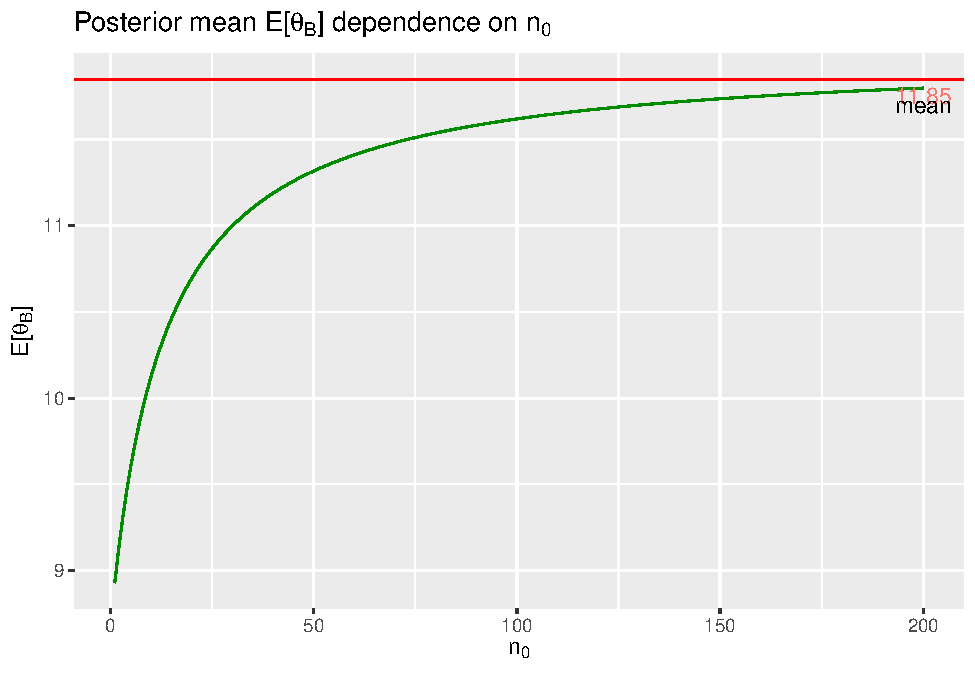
\includegraphics{2_hw_bs_code_files/figure-latex/unnamed-chunk-4-1.pdf}

\begin{Shaded}
\begin{Highlighting}[]
\NormalTok{p1 }\OtherTok{\textless{}{-}} \FunctionTok{mcmc\_trace}\NormalTok{(}\FunctionTok{as.data.frame}\NormalTok{(theta.mcmc), }\AttributeTok{pars =} \FunctionTok{c}\NormalTok{(}\StringTok{"V5"}\NormalTok{, }\StringTok{"V6"}\NormalTok{, }\StringTok{"V7"}\NormalTok{, }\StringTok{"V8"}\NormalTok{), }\AttributeTok{facet\_args =} \FunctionTok{list}\NormalTok{(}\AttributeTok{nrow =} \DecValTok{4}\NormalTok{, }\AttributeTok{labeller =}\NormalTok{ label\_parsed))}\SpecialCharTok{+}
  \FunctionTok{ggtitle}\NormalTok{(}\FunctionTok{expression}\NormalTok{(}\FunctionTok{paste}\NormalTok{(}\StringTok{"Traceplots of "}\NormalTok{, theta[}\DecValTok{5}\SpecialCharTok{:}\DecValTok{8}\NormalTok{])))}\SpecialCharTok{+}
  \FunctionTok{scale\_y\_continuous}\NormalTok{(}\AttributeTok{breaks =} \FunctionTok{c}\NormalTok{(}\DecValTok{4}\NormalTok{, }\DecValTok{6}\NormalTok{, }\DecValTok{8}\NormalTok{ ,}\DecValTok{10}\NormalTok{, }\DecValTok{12}\NormalTok{, }\DecValTok{14}\NormalTok{))}
\NormalTok{p2 }\OtherTok{\textless{}{-}} \FunctionTok{mcmc\_areas}\NormalTok{(}\FunctionTok{as.data.frame}\NormalTok{(theta.mcmc), }\AttributeTok{pars =} \FunctionTok{c}\NormalTok{(}\StringTok{"V5"}\NormalTok{, }\StringTok{"V6"}\NormalTok{, }\StringTok{"V7"}\NormalTok{, }\StringTok{"V8"}\NormalTok{), }\AttributeTok{prob =} \FloatTok{0.95}\NormalTok{, }
  \AttributeTok{prob\_outer =} \DecValTok{1}\NormalTok{,}
  \AttributeTok{point\_est =} \StringTok{"mean"}\NormalTok{) }\SpecialCharTok{+}
  \FunctionTok{ggtitle}\NormalTok{(}\FunctionTok{expression}\NormalTok{(}\FunctionTok{paste}\NormalTok{(}\StringTok{"Density plots of the posteriors for "}\NormalTok{, theta[}\DecValTok{5}\SpecialCharTok{:}\DecValTok{8}\NormalTok{])))}

\FunctionTok{grid.arrange}\NormalTok{(p1, p2, }\AttributeTok{nrow =} \DecValTok{1}\NormalTok{)}
\end{Highlighting}
\end{Shaded}

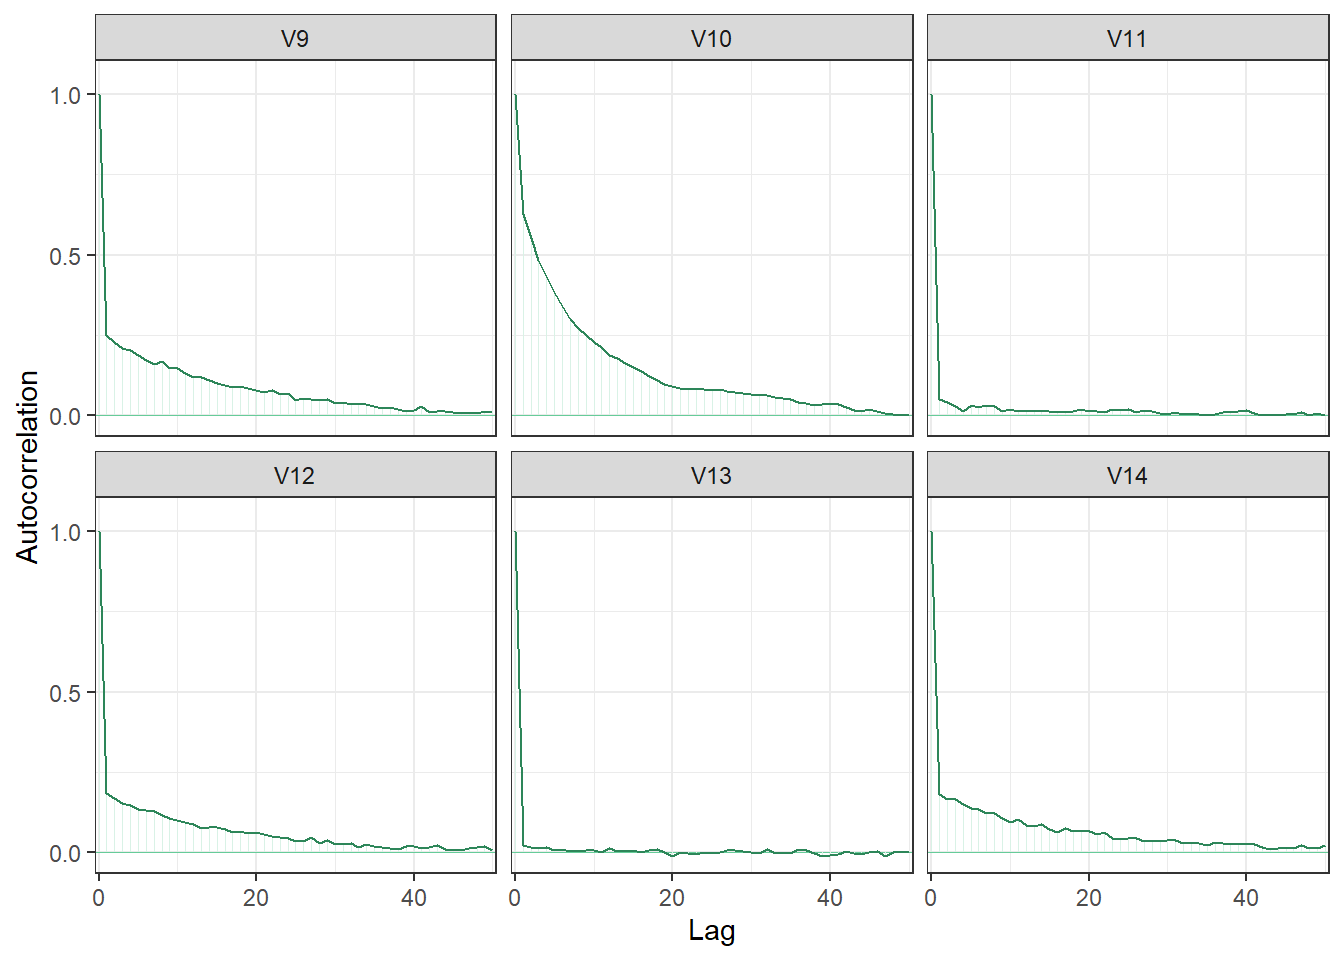
\includegraphics{2_hw_bs_code_files/figure-latex/unnamed-chunk-4-2.pdf}

\begin{Shaded}
\begin{Highlighting}[]
\CommentTok{\#comparison}
\FunctionTok{theme\_update}\NormalTok{(}\AttributeTok{plot.title =} \FunctionTok{element\_text}\NormalTok{(}\AttributeTok{hjust =} \FloatTok{0.5}\NormalTok{))}
\FunctionTok{color\_scheme\_set}\NormalTok{(}\StringTok{"purple"}\NormalTok{)}
\NormalTok{q1 }\OtherTok{\textless{}{-}} \FunctionTok{mcmc\_trace}\NormalTok{(}\FunctionTok{as.data.frame}\NormalTok{(mu.mcmc))}\SpecialCharTok{+}
  \FunctionTok{ggtitle}\NormalTok{(}\FunctionTok{expression}\NormalTok{(mu))}\SpecialCharTok{+}
  \FunctionTok{yaxis\_title}\NormalTok{(}\AttributeTok{on =} \ConstantTok{FALSE}\NormalTok{)}
\NormalTok{q2}\OtherTok{\textless{}{-}} \FunctionTok{mcmc\_areas}\NormalTok{(}
  \FunctionTok{as.data.frame}\NormalTok{(mu.mcmc), }
  \AttributeTok{prob =} \FloatTok{0.95}\NormalTok{,}
  \AttributeTok{prob\_outer =} \DecValTok{1}\NormalTok{, }
  \AttributeTok{point\_est =} \StringTok{"mean"}\NormalTok{)}\SpecialCharTok{+}
  \FunctionTok{ggtitle}\NormalTok{(}\FunctionTok{expression}\NormalTok{(mu))}\SpecialCharTok{+}
  \FunctionTok{yaxis\_text}\NormalTok{(}\AttributeTok{on =} \ConstantTok{FALSE}\NormalTok{)}

\FunctionTok{color\_scheme\_set}\NormalTok{(}\StringTok{"red"}\NormalTok{)}
\NormalTok{q3 }\OtherTok{\textless{}{-}} \FunctionTok{mcmc\_trace}\NormalTok{(}\FunctionTok{as.data.frame}\NormalTok{(sigma2.mcmc))}\SpecialCharTok{+}
  \FunctionTok{ggtitle}\NormalTok{(}\FunctionTok{expression}\NormalTok{(sigma}\SpecialCharTok{\^{}}\DecValTok{2}\NormalTok{))}\SpecialCharTok{+}
  \FunctionTok{yaxis\_title}\NormalTok{(}\AttributeTok{on =} \ConstantTok{FALSE}\NormalTok{)}
\NormalTok{q4 }\OtherTok{\textless{}{-}} \FunctionTok{mcmc\_areas}\NormalTok{(}
  \FunctionTok{as.data.frame}\NormalTok{(sigma2.mcmc), }
  \AttributeTok{prob =} \FloatTok{0.95}\NormalTok{, }
  \AttributeTok{prob\_outer =} \DecValTok{1}\NormalTok{, }
  \AttributeTok{point\_est =} \StringTok{"mean"}\NormalTok{)}\SpecialCharTok{+}
  \FunctionTok{ggtitle}\NormalTok{(}\FunctionTok{expression}\NormalTok{(sigma}\SpecialCharTok{\^{}}\DecValTok{2}\NormalTok{))}\SpecialCharTok{+}
  \FunctionTok{yaxis\_text}\NormalTok{(}\AttributeTok{on =} \ConstantTok{FALSE}\NormalTok{)}

\FunctionTok{color\_scheme\_set}\NormalTok{(}\StringTok{"teal"}\NormalTok{)}
\NormalTok{q5 }\OtherTok{\textless{}{-}} \FunctionTok{mcmc\_trace}\NormalTok{(}\FunctionTok{as.data.frame}\NormalTok{(tau2.mcmc))}\SpecialCharTok{+}
  \FunctionTok{ggtitle}\NormalTok{(}\FunctionTok{expression}\NormalTok{(tau}\SpecialCharTok{\^{}}\DecValTok{2}\NormalTok{))}\SpecialCharTok{+}
  \FunctionTok{yaxis\_title}\NormalTok{(}\AttributeTok{on =} \ConstantTok{FALSE}\NormalTok{)}
\NormalTok{q6 }\OtherTok{\textless{}{-}} \FunctionTok{mcmc\_areas}\NormalTok{(}
  \FunctionTok{as.data.frame}\NormalTok{(tau2.mcmc), }
  \AttributeTok{prob =} \FloatTok{0.95}\NormalTok{, }
  \AttributeTok{prob\_outer =} \DecValTok{1}\NormalTok{, }
  \AttributeTok{point\_est =} \StringTok{"mean"}\NormalTok{)}\SpecialCharTok{+}
  \FunctionTok{ggtitle}\NormalTok{(}\FunctionTok{expression}\NormalTok{(tau}\SpecialCharTok{\^{}}\DecValTok{2}\NormalTok{))}\SpecialCharTok{+}
  \FunctionTok{yaxis\_text}\NormalTok{(}\AttributeTok{on =} \ConstantTok{FALSE}\NormalTok{)}

\FunctionTok{grid.arrange}\NormalTok{(q1, q2, q3, q4, q5, q6, }\AttributeTok{nrow =} \DecValTok{3}\NormalTok{, }\AttributeTok{top=}\FunctionTok{textGrob}\NormalTok{(}\StringTok{"Traceplots and density plots"}\NormalTok{))}
\end{Highlighting}
\end{Shaded}

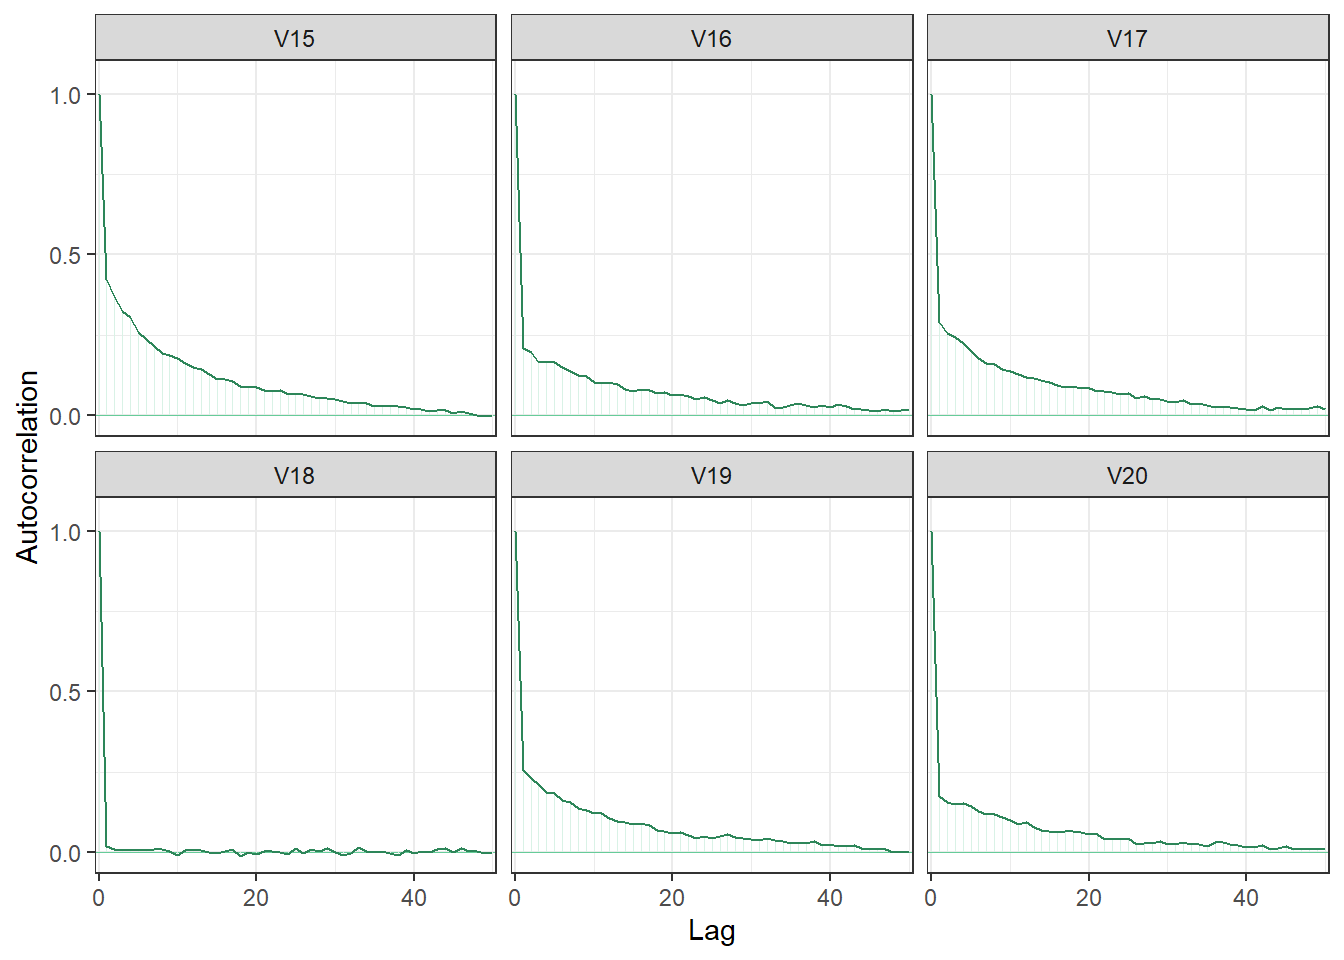
\includegraphics{2_hw_bs_code_files/figure-latex/unnamed-chunk-4-3.pdf}
\normalsize

\hypertarget{point-b.-1}{%
\subsection{Point b.}\label{point-b.-1}}

Therefore we can obtain the 95\%-quantile confidence regions of the
posterior densities for each parameter.

\scriptsize

\begin{Shaded}
\begin{Highlighting}[]
\FunctionTok{library}\NormalTok{(invgamma)}
\CommentTok{\#quantile{-}based 95\% confidence regions for the MCMC}
\NormalTok{alpha }\OtherTok{=} \FloatTok{0.05}

\NormalTok{a\_mu }\OtherTok{=} \FunctionTok{summary}\NormalTok{(mu.mcmc, }\AttributeTok{quantiles=} \FunctionTok{c}\NormalTok{(alpha}\SpecialCharTok{/}\DecValTok{2}\NormalTok{, }\DecValTok{1}\SpecialCharTok{{-}}\NormalTok{alpha}\SpecialCharTok{/}\DecValTok{2}\NormalTok{))}
\FunctionTok{print}\NormalTok{(}\FunctionTok{paste}\NormalTok{(}\StringTok{"The quantile{-}based 95\%{-}confidence region for mu is ["}\NormalTok{, a\_mu}\SpecialCharTok{$}\NormalTok{quantiles[}\DecValTok{1}\NormalTok{], }\StringTok{","}\NormalTok{, a\_mu}\SpecialCharTok{$}\NormalTok{quantiles[}\DecValTok{2}\NormalTok{], }\StringTok{"] and the posterior mean is "}\NormalTok{, a\_mu}\SpecialCharTok{$}\NormalTok{statistics[}\DecValTok{1}\NormalTok{]))}
\end{Highlighting}
\end{Shaded}

\begin{verbatim}
## [1] "The quantile-based 95%-confidence region for mu is [ 6.05099577534956 , 9.11350999134755 ] and the posterior mean is  7.57844639522663"
\end{verbatim}

\begin{Shaded}
\begin{Highlighting}[]
\NormalTok{a\_sigma }\OtherTok{=} \FunctionTok{summary}\NormalTok{(sigma2.mcmc, }\AttributeTok{quantiles=} \FunctionTok{c}\NormalTok{(alpha}\SpecialCharTok{/}\DecValTok{2}\NormalTok{, }\DecValTok{1}\SpecialCharTok{{-}}\NormalTok{alpha}\SpecialCharTok{/}\DecValTok{2}\NormalTok{))}
\FunctionTok{print}\NormalTok{(}\FunctionTok{paste}\NormalTok{(}\StringTok{"The quantile{-}based 95\%{-}confidence region for sigma\^{}2 is ["}\NormalTok{, a\_sigma}\SpecialCharTok{$}\NormalTok{quantiles[}\DecValTok{1}\NormalTok{], }\StringTok{","}\NormalTok{, a\_sigma}\SpecialCharTok{$}\NormalTok{quantiles[}\DecValTok{2}\NormalTok{], }\StringTok{"] and the posterior mean is"}\NormalTok{, a\_sigma}\SpecialCharTok{$}\NormalTok{statistics[}\DecValTok{1}\NormalTok{]))}
\end{Highlighting}
\end{Shaded}

\begin{verbatim}
## [1] "The quantile-based 95%-confidence region for sigma^2 is [ 11.6912071248673 , 17.9929876607772 ] and the posterior mean is 14.4886988279386"
\end{verbatim}

\begin{Shaded}
\begin{Highlighting}[]
\NormalTok{a\_tau }\OtherTok{=} \FunctionTok{summary}\NormalTok{(tau2.mcmc, }\AttributeTok{quantiles=} \FunctionTok{c}\NormalTok{(alpha}\SpecialCharTok{/}\DecValTok{2}\NormalTok{, }\DecValTok{1}\SpecialCharTok{{-}}\NormalTok{alpha}\SpecialCharTok{/}\DecValTok{2}\NormalTok{))}
\FunctionTok{print}\NormalTok{(}\FunctionTok{paste}\NormalTok{(}\StringTok{"The quantile{-}based 95\%{-}confidence region for tau\^{}2 is ["}\NormalTok{, a\_tau}\SpecialCharTok{$}\NormalTok{quantiles[}\DecValTok{1}\NormalTok{], }\StringTok{","}\NormalTok{, a\_tau}\SpecialCharTok{$}\NormalTok{quantiles[}\DecValTok{2}\NormalTok{], }\StringTok{"] and the posterior mean is"}\NormalTok{, a\_tau}\SpecialCharTok{$}\NormalTok{statistics[}\DecValTok{1}\NormalTok{]))}
\end{Highlighting}
\end{Shaded}

\begin{verbatim}
## [1] "The quantile-based 95%-confidence region for tau^2 is [ 1.86296816063879 , 14.0038507066232 ] and the posterior mean is 5.38080953765745"
\end{verbatim}

\begin{Shaded}
\begin{Highlighting}[]
\CommentTok{\#density plots comparison}
\NormalTok{x1 }\OtherTok{=} \FunctionTok{seq}\NormalTok{(mu0 }\SpecialCharTok{{-}} \DecValTok{2}\SpecialCharTok{*}\NormalTok{g20,  mu0 }\SpecialCharTok{+} \DecValTok{2}\SpecialCharTok{*}\NormalTok{g20, }\AttributeTok{length =} \DecValTok{200}\NormalTok{)}
\NormalTok{x2 }\OtherTok{=} \FunctionTok{seq}\NormalTok{(}\FloatTok{0.00001}\NormalTok{,  }\DecValTok{60}\NormalTok{, }\AttributeTok{length =} \DecValTok{200}\NormalTok{)}
\NormalTok{x3 }\OtherTok{=} \FunctionTok{seq}\NormalTok{(a\_sigma}\SpecialCharTok{$}\NormalTok{quantiles[}\DecValTok{1}\NormalTok{] }\SpecialCharTok{{-}} \DecValTok{10}\NormalTok{,  }\DecValTok{50}\NormalTok{, }\AttributeTok{length =} \DecValTok{200}\NormalTok{)}
\NormalTok{norm\_vals }\OtherTok{=} \FunctionTok{dnorm}\NormalTok{(x1, mu0, g20)}
\NormalTok{invG\_tau }\OtherTok{=} \FunctionTok{dinvgamma}\NormalTok{(x2, eta0}\SpecialCharTok{/}\DecValTok{2}\NormalTok{, eta0}\SpecialCharTok{*}\NormalTok{t20}\SpecialCharTok{/}\DecValTok{2}\NormalTok{)}
\NormalTok{invG\_sigma }\OtherTok{=} \FunctionTok{dinvgamma}\NormalTok{(x3, nu0}\SpecialCharTok{/}\DecValTok{2}\NormalTok{, nu0}\SpecialCharTok{*}\NormalTok{s20}\SpecialCharTok{/}\DecValTok{2}\NormalTok{)}
\NormalTok{priors }\OtherTok{=} \FunctionTok{data.frame}\NormalTok{(x1, x2, x3, norm\_vals, invG\_sigma, invG\_tau)}

\FunctionTok{color\_scheme\_set}\NormalTok{(}\StringTok{"blue"}\NormalTok{)}
\FunctionTok{mcmc\_dens}\NormalTok{(}\FunctionTok{as.data.frame}\NormalTok{(mu.mcmc), }\AttributeTok{alpha =} \FloatTok{0.5}\NormalTok{)}\SpecialCharTok{+}
  \FunctionTok{xaxis\_text}\NormalTok{(}\AttributeTok{on =} \ConstantTok{FALSE}\NormalTok{)}\SpecialCharTok{+}
  \FunctionTok{ggtitle}\NormalTok{(}\FunctionTok{expression}\NormalTok{(}\FunctionTok{paste}\NormalTok{(}\StringTok{"Posterior distribution of "}\NormalTok{, mu))) }\SpecialCharTok{+}
  \FunctionTok{geom\_area}\NormalTok{(}\AttributeTok{data =}\NormalTok{ priors, }\FunctionTok{aes}\NormalTok{(}\AttributeTok{x=}\NormalTok{ x1, }\AttributeTok{y=}\NormalTok{norm\_vals, }\AttributeTok{col =} \StringTok{"prior"}\NormalTok{),  }\AttributeTok{fill =} \StringTok{"red"}\NormalTok{, }\AttributeTok{alpha =} \FloatTok{0.3}\NormalTok{, }\AttributeTok{size =} \FloatTok{0.8}\NormalTok{) }\SpecialCharTok{+}
  \FunctionTok{geom\_vline}\NormalTok{(}\FunctionTok{aes}\NormalTok{(}\AttributeTok{xintercept =}\NormalTok{ a\_mu}\SpecialCharTok{$}\NormalTok{statistics[}\DecValTok{1}\NormalTok{], }\AttributeTok{col =} \StringTok{"posterior"}\NormalTok{), }\AttributeTok{size =} \DecValTok{1}\NormalTok{)}\SpecialCharTok{+}
  \FunctionTok{geom\_vline}\NormalTok{(}\FunctionTok{aes}\NormalTok{(}\AttributeTok{xintercept =}\NormalTok{ mu0, }\AttributeTok{col =} \StringTok{"prior"}\NormalTok{), }\AttributeTok{size =} \DecValTok{1}\NormalTok{)}\SpecialCharTok{+}
  \FunctionTok{scale\_color\_manual}\NormalTok{(}\AttributeTok{name =} \StringTok{"Legend"}\NormalTok{, }\AttributeTok{values =} \FunctionTok{c}\NormalTok{(}\StringTok{"prior"} \OtherTok{=} \StringTok{"red"}\NormalTok{, }\StringTok{"posterior"} \OtherTok{=} \StringTok{"blue"}\NormalTok{), }
    \AttributeTok{labels =} \FunctionTok{c}\NormalTok{(}\StringTok{"prior distribution"}\NormalTok{, }\StringTok{"posterior distribution"}\NormalTok{))}
\end{Highlighting}
\end{Shaded}

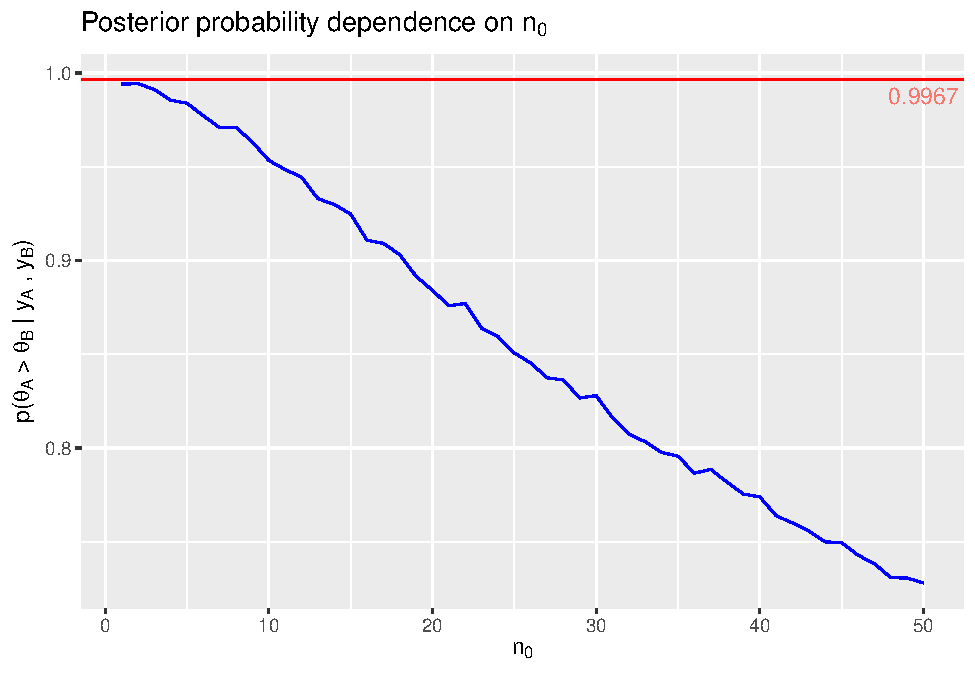
\includegraphics{2_hw_bs_code_files/figure-latex/unnamed-chunk-5-1.pdf}

\begin{Shaded}
\begin{Highlighting}[]
\FunctionTok{mcmc\_dens}\NormalTok{(}\FunctionTok{as.data.frame}\NormalTok{(tau2.mcmc), }\AttributeTok{alpha =} \FloatTok{0.5}\NormalTok{)}\SpecialCharTok{+}
  \FunctionTok{xaxis\_text}\NormalTok{(}\AttributeTok{on =} \ConstantTok{FALSE}\NormalTok{)}\SpecialCharTok{+}
  \FunctionTok{ggtitle}\NormalTok{(}\FunctionTok{expression}\NormalTok{(}\FunctionTok{paste}\NormalTok{(}\StringTok{"Posterior distribution of "}\NormalTok{, tau}\SpecialCharTok{\^{}}\DecValTok{2}\NormalTok{))) }\SpecialCharTok{+}
  \FunctionTok{geom\_area}\NormalTok{(}\AttributeTok{data =}\NormalTok{ priors, }\FunctionTok{aes}\NormalTok{(}\AttributeTok{x=}\NormalTok{ x2, }\AttributeTok{y=}\NormalTok{invG\_tau, }\AttributeTok{col =} \StringTok{"prior"}\NormalTok{), }\AttributeTok{fill =} \StringTok{"red"}\NormalTok{, }\AttributeTok{alpha =} \FloatTok{0.3}\NormalTok{, }\AttributeTok{size =} \FloatTok{0.8}\NormalTok{) }\SpecialCharTok{+}
  \FunctionTok{geom\_vline}\NormalTok{(}\FunctionTok{aes}\NormalTok{(}\AttributeTok{xintercept =}\NormalTok{ a\_tau}\SpecialCharTok{$}\NormalTok{statistics[}\DecValTok{1}\NormalTok{], }\AttributeTok{col =} \StringTok{"posterior"}\NormalTok{), }\AttributeTok{size =} \DecValTok{1}\NormalTok{)}\SpecialCharTok{+}
  \FunctionTok{geom\_vline}\NormalTok{(}\FunctionTok{aes}\NormalTok{(}\AttributeTok{xintercept =}\NormalTok{ t20, }\AttributeTok{col =} \StringTok{"prior"}\NormalTok{), }\AttributeTok{size =} \DecValTok{1}\NormalTok{)}\SpecialCharTok{+}
  \FunctionTok{scale\_color\_manual}\NormalTok{(}\AttributeTok{name =} \StringTok{"Legend"}\NormalTok{, }\AttributeTok{values =} \FunctionTok{c}\NormalTok{(}\StringTok{"prior"} \OtherTok{=} \StringTok{"red"}\NormalTok{, }\StringTok{"posterior"} \OtherTok{=} \StringTok{"blue"}\NormalTok{), }
    \AttributeTok{labels =} \FunctionTok{c}\NormalTok{(}\StringTok{"prior distribution"}\NormalTok{, }\StringTok{"posterior distribution"}\NormalTok{))}
\end{Highlighting}
\end{Shaded}

\includegraphics{2_hw_bs_code_files/figure-latex/unnamed-chunk-5-2.pdf}

\begin{Shaded}
\begin{Highlighting}[]
\FunctionTok{mcmc\_dens}\NormalTok{(}\FunctionTok{as.data.frame}\NormalTok{(sigma2.mcmc), }\AttributeTok{alpha =} \FloatTok{0.5}\NormalTok{)}\SpecialCharTok{+}
  \FunctionTok{xaxis\_text}\NormalTok{(}\AttributeTok{on =} \ConstantTok{FALSE}\NormalTok{)}\SpecialCharTok{+}
  \FunctionTok{ggtitle}\NormalTok{(}\FunctionTok{expression}\NormalTok{(}\FunctionTok{paste}\NormalTok{(}\StringTok{"Posterior distribution of "}\NormalTok{, sigma}\SpecialCharTok{\^{}}\DecValTok{2}\NormalTok{))) }\SpecialCharTok{+}
  \FunctionTok{geom\_area}\NormalTok{(}\AttributeTok{data =}\NormalTok{ priors, }\FunctionTok{aes}\NormalTok{(}\AttributeTok{x=}\NormalTok{ x3, }\AttributeTok{y=}\NormalTok{invG\_sigma, }\AttributeTok{col =} \StringTok{"prior"}\NormalTok{), }\AttributeTok{fill =} \StringTok{"red"}\NormalTok{, }\AttributeTok{alpha =} \FloatTok{0.3}\NormalTok{, }\AttributeTok{size =} \FloatTok{0.8}\NormalTok{) }\SpecialCharTok{+}
  \FunctionTok{geom\_vline}\NormalTok{(}\FunctionTok{aes}\NormalTok{(}\AttributeTok{xintercept =}\NormalTok{ a\_sigma}\SpecialCharTok{$}\NormalTok{statistics[}\DecValTok{1}\NormalTok{], }\AttributeTok{col =} \StringTok{"posterior"}\NormalTok{), }\AttributeTok{size =} \DecValTok{1}\NormalTok{)}\SpecialCharTok{+}
  \FunctionTok{geom\_vline}\NormalTok{(}\FunctionTok{aes}\NormalTok{(}\AttributeTok{xintercept =}\NormalTok{ s20, }\AttributeTok{col =} \StringTok{"prior"}\NormalTok{), }\AttributeTok{size =} \DecValTok{1}\NormalTok{)}\SpecialCharTok{+}
  \FunctionTok{scale\_color\_manual}\NormalTok{(}\AttributeTok{name =} \StringTok{"Legend"}\NormalTok{, }\AttributeTok{values =} \FunctionTok{c}\NormalTok{(}\StringTok{"prior"} \OtherTok{=} \StringTok{"red"}\NormalTok{, }\StringTok{"posterior"} \OtherTok{=} \StringTok{"blue"}\NormalTok{), }
    \AttributeTok{labels =} \FunctionTok{c}\NormalTok{(}\StringTok{"prior distribution"}\NormalTok{, }\StringTok{"posterior distribution"}\NormalTok{))}
\end{Highlighting}
\end{Shaded}

\includegraphics{2_hw_bs_code_files/figure-latex/unnamed-chunk-5-3.pdf}
\normalsize

\hypertarget{point-c.-1}{%
\subsection{Point c.}\label{point-c.-1}}

\scriptsize

\normalsize

\hypertarget{point-d.-1}{%
\subsection{Point d.}\label{point-d.-1}}

\scriptsize

\begin{Shaded}
\begin{Highlighting}[]
\NormalTok{a\_theta }\OtherTok{=} \FunctionTok{summary}\NormalTok{(theta.mcmc)}
\NormalTok{post\_means }\OtherTok{=}\NormalTok{ a\_theta}\SpecialCharTok{$}\NormalTok{statistics[}\DecValTok{1}\SpecialCharTok{:}\DecValTok{8}\NormalTok{, }\DecValTok{1}\NormalTok{]}

\NormalTok{sample.theta9 }\OtherTok{=}  \FunctionTok{rep}\NormalTok{(}\DecValTok{0}\NormalTok{, S)}
\NormalTok{sample.y7 }\OtherTok{=}  \FunctionTok{rep}\NormalTok{(}\DecValTok{0}\NormalTok{, S)}
\NormalTok{sample.y9 }\OtherTok{=}  \FunctionTok{rep}\NormalTok{(}\DecValTok{0}\NormalTok{, S)}
  
\ControlFlowTok{for}\NormalTok{ (i }\ControlFlowTok{in} \DecValTok{1}\SpecialCharTok{:}\NormalTok{S)\{}
\NormalTok{  sample.theta9[i] }\OtherTok{=} \FunctionTok{rnorm}\NormalTok{(}\DecValTok{1}\NormalTok{, mu, }\FunctionTok{sqrt}\NormalTok{(tau2.mcmc[i, }\AttributeTok{drop =} \ConstantTok{TRUE}\NormalTok{]))}
\NormalTok{  sample.y7[i] }\OtherTok{=} \FunctionTok{rnorm}\NormalTok{(}\DecValTok{1}\NormalTok{, theta.mcmc[i, }\DecValTok{7}\NormalTok{, }\AttributeTok{drop =} \ConstantTok{TRUE}\NormalTok{], }\FunctionTok{sqrt}\NormalTok{(sigma2.mcmc[i, }\AttributeTok{drop =} \ConstantTok{TRUE}\NormalTok{]))}
\NormalTok{  sample.y9[i] }\OtherTok{=} \FunctionTok{rnorm}\NormalTok{(}\DecValTok{1}\NormalTok{, sample.theta9[i], }\FunctionTok{sqrt}\NormalTok{(sigma2.mcmc[i, }\AttributeTok{drop =} \ConstantTok{TRUE}\NormalTok{]))}
\NormalTok{\}}

\NormalTok{mc\_theta }\OtherTok{=} \FunctionTok{sum}\NormalTok{(sample.theta9 }\SpecialCharTok{\textgreater{}}\NormalTok{ theta.mcmc[}\DecValTok{1}\SpecialCharTok{:}\NormalTok{S, }\DecValTok{7}\NormalTok{]) }\SpecialCharTok{/}\NormalTok{ S}
\NormalTok{mc\_y }\OtherTok{=} \FunctionTok{sum}\NormalTok{(sample.y9 }\SpecialCharTok{\textgreater{}}\NormalTok{ sample.y7)}\SpecialCharTok{/}\NormalTok{S}
\FunctionTok{writeLines}\NormalTok{(}\FunctionTok{paste}\NormalTok{(}\StringTok{"The Monte Carlo estimate of the posterior probability of \{theta9 \textgreater{} theta7\} is:"}\NormalTok{, mc\_theta, }\StringTok{"}\SpecialCharTok{\textbackslash{}n}\StringTok{The Monte Carlo estimate of the posterior predictive probability of \{Y9 \textgreater{} Y7\} is:"}\NormalTok{, mc\_y))}
\end{Highlighting}
\end{Shaded}

\begin{verbatim}
## The Monte Carlo estimate of the posterior probability of {theta9 > theta7} is: 0.8128 
## The Monte Carlo estimate of the posterior predictive probability of {Y9 > Y7} is: 0.6484
\end{verbatim}

\normalsize

\hypertarget{point-e.}{%
\subsection{Point e.}\label{point-e.}}

\scriptsize

\begin{Shaded}
\begin{Highlighting}[]
\FunctionTok{library}\NormalTok{(ggrepel)}

\NormalTok{mean\_plt }\OtherTok{=} \FunctionTok{data.frame}\NormalTok{(post\_means, ybar, }\AttributeTok{names =} \DecValTok{1}\SpecialCharTok{:}\DecValTok{8}\NormalTok{)}

\NormalTok{mean\_plt }\SpecialCharTok{\%\textgreater{}\%} \FunctionTok{ggplot}\NormalTok{(}\FunctionTok{aes}\NormalTok{(}\AttributeTok{x=}\NormalTok{post\_means, }\AttributeTok{y =}\NormalTok{ ybar))}\SpecialCharTok{+}
  \FunctionTok{geom\_point}\NormalTok{( }\AttributeTok{col =} \StringTok{"green"}\NormalTok{)}\SpecialCharTok{+}
  \FunctionTok{geom\_line}\NormalTok{(}\AttributeTok{col =} \StringTok{"darkgreen"}\NormalTok{, }\AttributeTok{alpha =} \FloatTok{0.5}\NormalTok{)}\SpecialCharTok{+}
  \FunctionTok{ylab}\NormalTok{(}\FunctionTok{expression}\NormalTok{(y[i])) }\SpecialCharTok{+}
  \FunctionTok{xlab}\NormalTok{(}\FunctionTok{expression}\NormalTok{(}\FunctionTok{paste}\NormalTok{(theta[i]))) }\SpecialCharTok{+}
  \FunctionTok{ggtitle}\NormalTok{(}\FunctionTok{expression}\NormalTok{(}\FunctionTok{paste}\NormalTok{(}\StringTok{"Posterior mean parameters "}\NormalTok{, theta[i], }\StringTok{" VS sample means "}\NormalTok{, y[i])))}\SpecialCharTok{+}
  \FunctionTok{scale\_color\_discrete}\NormalTok{(}\AttributeTok{guide =} \StringTok{"none"}\NormalTok{)}\SpecialCharTok{+}
  \FunctionTok{geom\_label\_repel}\NormalTok{(}\FunctionTok{aes}\NormalTok{(}\AttributeTok{label =}\NormalTok{ names),}
                  \AttributeTok{box.padding   =} \FloatTok{0.35}\NormalTok{, }
                  \AttributeTok{point.padding =} \FloatTok{0.5}\NormalTok{,}
                  \AttributeTok{segment.color =} \StringTok{\textquotesingle{}grey50\textquotesingle{}}\NormalTok{)}
\end{Highlighting}
\end{Shaded}

\includegraphics{2_hw_bs_code_files/figure-latex/unnamed-chunk-8-1.pdf}

\begin{Shaded}
\begin{Highlighting}[]
\NormalTok{total.sample.mean }\OtherTok{=} \FunctionTok{sum}\NormalTok{(n}\SpecialCharTok{*}\NormalTok{ybar)}\SpecialCharTok{/}\FunctionTok{sum}\NormalTok{(n)}

\FunctionTok{writeLines}\NormalTok{(}\FunctionTok{paste}\NormalTok{(}\StringTok{"The total sample mean is: "}\NormalTok{, }\FunctionTok{round}\NormalTok{(total.sample.mean, }\DecValTok{2}\NormalTok{), }\StringTok{"}\SpecialCharTok{\textbackslash{}n}\StringTok{The posterior expectation of the Grand Mean is: "}\NormalTok{, }\FunctionTok{round}\NormalTok{(a\_mu}\SpecialCharTok{$}\NormalTok{statistics[}\DecValTok{1}\NormalTok{], }\DecValTok{2}\NormalTok{), }\StringTok{"}\SpecialCharTok{\textbackslash{}n}\StringTok{So they only differ by "}\NormalTok{, }\FunctionTok{round}\NormalTok{(}\FunctionTok{abs}\NormalTok{(a\_mu}\SpecialCharTok{$}\NormalTok{statistics[}\DecValTok{1}\NormalTok{] }\SpecialCharTok{{-}}\NormalTok{ total.sample.mean)}\SpecialCharTok{/}\NormalTok{total.sample.mean }\SpecialCharTok{*}\DecValTok{100}\NormalTok{, }\DecValTok{2}\NormalTok{), }\StringTok{"\% of the former"}\NormalTok{))}
\end{Highlighting}
\end{Shaded}

\begin{verbatim}
## The total sample mean is:  7.69 
## The posterior expectation of the Grand Mean is:  7.58 
## So they only differ by  1.47 % of the former
\end{verbatim}

\end{document}
